\documentclass{article}
%\usepackage{ctex} %Chinese
\usepackage{float} %H-float
\usepackage{graphicx} %
\usepackage{amsmath} %
\usepackage{amssymb} %
\usepackage{amsthm} %
\usepackage{mathtools}
\usepackage{caption}
\usepackage[version=3]{mhchem}  %
\usepackage{chemfig}    %
\usepackage{physics}
\usepackage{booktabs}
\usepackage{hyperref}
%\usepackage{caption}    %
%  \captionsetup[figure]{name=Fig}
\usepackage{enumerate} %列表
\usepackage[scale=0.85]{geometry} %
\usepackage{tikz}
%\usepackage{mmap}
%\usepackage{tikz,venndiagram}
\newtheorem{theorem}{Theorem}
\newtheorem{corollary}{Corollary}[theorem]
\newtheorem{lemma}[theorem]{Lemma}

\newcommand{\sq}[1]{\ensuremath{\left[{#1}\right]}}
\newcommand{\R}[1]{\ensuremath{\mathrm{R}\!\left({#1}\right)}}
\newcommand{\kB}{\ensuremath{k_\mathrm{B}}}
\newcommand{\iu}{\ensuremath{\mathrm{i}}}
\newcommand{\dpath}[1]{\ensuremath{\mathcal{D}\!\left[{#1}\right]}}
\newcommand{\set}[1]{\ensuremath{\left\{{#1}\right\}}}
\newcommand{\kket}[1]{\ensuremath{\ket{\ket{#1}}}}
\newcommand{\ie}{\emph{i.\,e.}}

\DeclareFontFamily{OMS}{oasy}{\skewchar\font48 }
\DeclareFontShape{OMS}{oasy}{m}{n}{%
         <-5.5> oasy5     <5.5-6.5> oasy6
      <6.5-7.5> oasy7     <7.5-8.5> oasy8
      <8.5-9.5> oasy9     <9.5->  oasy10
      }{}
\DeclareFontShape{OMS}{oasy}{b}{n}{%
       <-6> oabsy5
      <6-8> oabsy7
      <8->  oabsy10
      }{}
\DeclareSymbolFont{oasy}{OMS}{oasy}{m}{n}
\SetSymbolFont{oasy}{bold}{OMS}{oasy}{b}{n}

\DeclareMathSymbol{\smallleftarrow}     {\mathrel}{oasy}{"20}
\DeclareMathSymbol{\smallrightarrow}    {\mathrel}{oasy}{"21}
\DeclareMathSymbol{\smallleftrightarrow}{\mathrel}{oasy}{"24}

\newcommand{\tensor}[1]{\overset{\scriptscriptstyle\smallleftrightarrow}{#1}}



\title{CHM452: Problem Set 2}
\author{Xinxian Chen%
\footnote{Email: \href{mailto:xchen106@ur.rochester.edu}{xchen106@ur.rochester.edu}}}
\date{\today}

\begin{document}

\maketitle

Let $\iu = \sqrt{-1}$, $o(\cdot)$ and $O(\cdot)$ are little-o and big-O notations, respectively, and $\mathbb{N}$ is the set of natural numbers ($\mathbb{N} = \set{0,\ 1,\ 2,\ 3,\ \ldots}$) and $\mathbb{N}_+ = \mathbb{N}\setminus\set{0}$

\begin{enumerate}[1.]
  \item 
  \begin{enumerate}[(i)]
    \item Since $\Psi(x,\ t)$ is a linear combination of $\Phi_n(x,\ t)$, where
    \begin{align*}
      \Phi_n(x,\ t) = \sqrt{\frac{2}{w}}\sin\qty(\frac{n\pi}{w(t)}x)\exp\qty(\frac{\iu\qty(mvx^2 - 2E_n^iat)}{2\hbar w(t)}),
    \end{align*}
    $w(t) =a + vt$, and $E_n^i = n^2\pi^2\hbar^2/2ma^2$, we only need to check that $\Phi_n(x,\ t)$ satisfies the boundary condition for all $n \in \mathbb{N}_+$
    \begin{align*}
      \Phi_n(x=0,\ t) = 0, \qquad \Phi_n(x=w(t),\ t) = 0.
    \end{align*}
    On the other hand,
    \begin{align*}
      \Phi_n(x=0,\ t) &= \sqrt{\frac{2}{w}}\sin\qty(\frac{n\pi}{w(t)} \cdot 0)\exp\qty(\frac{\iu\qty(- 2E_n^iat)}{2\hbar w(t)}) = 0,\\
      \Phi_n(x=w(t),\ t) &= \sqrt{\frac{2}{w}}\sin\qty(\frac{n\pi}{w(t)} w(t))\exp\qty(\frac{\iu\qty(mvw^2 - 2E_n^iat)}{2\hbar w(t)}) \\
      &=\sqrt{\frac{2}{w}}\sin\qty(n \pi)\exp\qty(\frac{\iu\qty(mvw^2 - 2E_n^iat)}{2\hbar w(t)}) = 0.
    \end{align*}
    Therefore, $\Phi_n(x,\ t)$ satisfies the boundary conditions, and hence, $\Psi(x,\ t)$ satisfies the boundary conditions.
    \item At $t=0$,
    \begin{align*}
      c_n =& \int_0^a \Phi_n(x,\ 0)^* \Psi(x,\ 0) \dd{x} = \int_0^a \qty( \sqrt{\frac{2}{a}}\sin\qty(\frac{n\pi}{a}x)e^{\frac{\iu mvx^2}{2\hbar a}})^*  \sqrt{\frac{2}{a}}\sin\qty(\frac{\pi x}{a}) \dd{x}\\
      =& \frac{2}{a} \int_0^a \sin\qty(n\frac{\pi x}{a})e^{-\iu\frac{mva}{2\pi^2\hbar} \qty(\frac{\pi x}{a})^2} \sin\qty(\frac{\pi x}{a}) \dd{x}.
    \end{align*}
    Let $z = \pi x /a$, then
    \begin{align*}
      c_n =& \frac{2}{a} \int_0^\pi \sin\qty(nz) e^{-\iu\frac{mva}{2\pi^2\hbar}z^2} \sin\qty(z) \dv{x}{z}\dd{z} = \frac{2}{\pi} \int_0^\pi e^{-\iu\alpha z^2} \sin\qty(nz) \sin\qty(z) \dd{z},
    \end{align*}
    where $\alpha = \frac{mva}{2\pi^2\hbar}$.
    \item 
    Without loss of generality, suppose the initial time is at $t = 0$ and the final time is at $t = \Delta t$.
    For the instantaneous eigenstate $\psi_n(x,\ t)$ at time $t$, it satisfies the TISE at some specific time
    \begin{align*}
      -\frac{\hbar^2}{2m}\dv[2]{x}\psi_n(x,\ t) = E_n(t) \psi_n(x,\ t),
    \end{align*}
    and it satisfies the boundary conditions at time $t$:
    \begin{align*}
      \psi_n(x=0,\ t) = 0, \qquad \psi_n(x=w(t),\ t) = 0.
    \end{align*}
    Solve the ODE and we have that $\psi_n(x,\ t) = N\sin\qty(\frac{n\pi x}{w(t)})$ and $E_n(t) = n^2\pi^2\hbar^2/2mw(t)^2$; if we require the instantaneous eigenstates are orthonormal, \emph{i.\,e.}, $\int_0^{w(t)} \psi_n(x,\ t)^* \psi_m(x,\ t)  \dd{x} = \delta_{nm}$, then we have that $N = \sqrt{2/w(t)}$, and hence, 
    \begin{align*}
      \psi_n(x,\ t) = \sqrt{\frac{2}{w(t)}}\sin\qty(\frac{n\pi x}{w(t)}).
    \end{align*}
    Now we can use the instantaneous eigenstates to represent the solution
    \begin{align*}
      \Psi (x,\ t) = \sum_{n=1}^\infty a_n(t)\psi_{n}(x,\ t) e^{\iu\theta_{n}(t)},
    \end{align*}
    where $\theta_n = -\int_0^t E_n(t')/\hbar \dd{t'}$.
    From the adiabatic theorem, we have that
    \begin{align*}
      \dv{t} a_n(t) \approx& -a_n(t) \int_0^{w(t)} \psi_{n}(x,\ t) \dv{t} \psi_{n}(x,\ t) \dd{x}\\
      =&  -a_n(t) \frac{2}{w(t)} \frac{n\pi}{w(t)} \int_0^{w(t)} \sin\qty(\frac{n\pi x}{w(t)})\cos\qty(\frac{n\pi x}{w(t)}) \dd{x} 
      =0.
    \end{align*}
    On the other hand, at $t = 0$, we have that $a_n(0) = \delta_{1n}$. Therefore,
    \begin{align*}
      a_n(t) = \delta_{1n}.
    \end{align*}
    Note that the well expands to twice its original time in a time $\Delta t$, which means $v = a/\Delta t$. Therefore,
    \begin{align*}
      \Psi(x,\ t) = a_1(t)\psi_{1}(x,\ t) e^{\iu\theta_{1}(t)} = e^{\iu\theta(t)} \sqrt{\frac{2}{w(t)}}\sin\qty(\frac{\pi x}{w(t)}),
    \end{align*}
    where $w(t) = a(1+t/\Delta t)$ and 
    \begin{align*}
      \theta(t) = -\frac{1}{\hbar} \int_0^t \frac{\pi^2\hbar^2}{2ma^2(1+t'/\Delta t)^2}\dd{t'} = -\frac{\pi^2\hbar}{2ma^2} \frac{t}{1 + t/\Delta t}. 
    \end{align*}

    On the other hand, if the velocity of expansion $v$ is small enough, \emph{i.\,e.}, $v \to 0$, from the exact solution, we will have that $\alpha = mva/2\pi^2\hbar \approx 0$ and
    \begin{align*}
      c_n(t) \approx \frac{2}{\pi}\int_0^\pi \sin(nz)\sin(z)\dd{z} = \delta_{1n}.
    \end{align*} 
    Hence,
    \begin{align*}
      \Psi(x,\ t) =& \sum_{i=1}^\infty c_n(t)\Phi_n(x,\ t) \approx \Phi_1(x,\ t) =  \sqrt{\frac{2}{w}}\sin\qty(\frac{\pi}{w(t)}x)\exp\qty(\frac{\iu\qty(mvx^2 - 2E_1^iat)}{2\hbar w(t)})
      \\ =&  e^{\iu\theta'(t)} \sqrt{\frac{2}{w}}\sin\qty(\frac{\pi}{w(t)}x),
    \end{align*}
    where $\theta'(t) = \frac{mvx^2 - 2E_1^iat}{2\hbar w(t)} \approx - \frac{\pi^2\hbar^2at}{2ma^2\hbar a(1 + t/\Delta t)} = -\frac{\pi^2\hbar a t}{2ma^2 (1 + t/\Delta t)}$, which is consistent with the result from the adiabatic theorem at the limit of $v \to 0$.
    \item If the expansion of the well can be considered as a sudden perturbation, that is, the stationary state does not change as $t$ goes from $0$ to $\Delta t$, that is, $\Psi(x,\ \Delta t) \approx \Psi(x,\ 0) = \sqrt{2/a}\sin(\pi x / a)$;
    
    On the other hand, since $\comm{H(t_1)}{H(t_2)} = 0$ for all $t_1,\ t_2 \in [0,\ \Delta t]$,
    \begin{align*}
      \Psi(x,\ \Delta t) = e^{-\iu \bar{H} \Delta t/\hbar} \sum_{n=1}^\infty c_n \Phi_n (x,\ 0) = e^{-\iu E^i t/\hbar}\sum_{n=1}^\infty c_n e^{-\iu(E_n - E^i)t/\hbar} \Phi_n (x,\ 0).
    \end{align*} 
    where $E^i$ is the energy at initial state. Notice that only terms satisfying $t > \hbar/(E_n - E^i)$ will make appreciable change, and for the sudden perturbation limit, we hence require $t \ll \hbar/(E_n - E^i)$ for all $n$, that is, $t \ll \hbar/\Delta \bar{H}$.
  \end{enumerate}

  \item Landau--Zener theory gives a formula that predicts the nonadiabatic transit possibility. If the hamiltonian is
  \begin{align*}
    H =& H_0 + V, \\
    H_0 =& E_1(t)\op{1} + E_2(t)\op{2}, \\
    V =& \frac{\Delta}{2}\op{1}{2} + \frac{\Delta}{2}\op{1}{2},
  \end{align*}
  where $E_1(t) = vt/2$, $E_2(t) = -vt/2$,  and we start with $\ket{(\psi(t=-\infty))} = \ket{1}$, then for $t \to +\infty$, Laudau--Zener theory gives the nonadiabatic transit possibility
  \begin{align*}
    P_{1\to 2} = 1-e^{\frac{\Delta^2\pi}{2\hbar v}}.
  \end{align*}
  For instance, for the molecular dynamics Laudau--Zener indicates that the nonadiabatic transitions take place only when the surface gap attains a local minimum for each classical trajectory, which gives the theoretical basis of surface hopping algorithms.

  \item
  \begin{enumerate}[(i)]
    \item The Floquet Hamiltonian is
    \begin{align*}
      \mathcal{H} = H(t) - \iu\hbar\pdv{t}
    \end{align*}
    The Floquet Hamiltonian is defined on the expanded Hilbert space that spanned by basis $\set{\ket{\alpha n}} \coloneqq \set{\ket{\alpha}\ket{n}}$, where $\ket{\alpha} \in \set{\ket{E_1},\ \ket{E_2}}$ and $\ip{t}{n} = e^{\iu n \omega t}$. 
    The Floquet mode $\ket{U_\lambda}$ satisfies
    \begin{align*}
      \mathcal{H} \ket{U_\lambda} = \mathcal{E}_\lambda \ket{U_\lambda}.
    \end{align*}
    Let
    \begin{align*}
      {\ip{\beta t}{U_\lambda}} =& \sum_{m=-\infty}^\infty U_{\beta\lambda}^{(m)}e^{\iu m \omega t},\\
      \mel{\alpha}{H(t)}{\beta} =& \sum_{n = -\infty}^{\infty} H_{\alpha\beta}^{(n)}e^{\iu n \omega t}.
    \end{align*}
    Then,
    \begin{align*}
      {\mel{\alpha m }{\mathcal{H}}{\beta n}} = \sum_k H_{\alpha\beta}^{(k)} \frac{1}{T}\int_0^T e^{\iu (k-m+n) \omega t} + n\hbar\omega\delta_{\alpha\beta}\delta_{mn} = H_{\alpha\beta}^{(m-n)} + n\hbar\omega\delta_{\alpha\beta}\delta_{mn} 
    \end{align*}
    where $T = 2\pi / \omega$. 
    On the other hand, from the matrix representation of $H(t)$ we have that 
    \begin{align*}
      H^{(0)} =& \mqty(-\hbar\omega_0/2 & \\ & \hbar\omega_0/2), \\
      H^{(-1)} =& \mqty( & b \\ b & ), \\
      H^{(1)} =& \mqty( & b \\ b & ), \\
      H^{(n)} =& 0, \text{ otherwise.}
    \end{align*}
    where we have applied the fact that $\cos\omega t = \qty(e^{\iu\omega t} + e^{-\iu\omega t})/2$.
    Therefore, the matrix representation of $\mathcal{H}$ under basis $\set{\kket{\alpha n}}$ is
    \begin{align*}
      \mqty(
        \ddots & \ddots           &   &                 &        \\
        \ddots & A - \hbar\omega  & B &                 &        \\
               & B                & A & B               &        \\
               &                  & B & A + \hbar\omega & \ddots \\
               &                  &   & \ddots          & \ddots
        ),
    \end{align*}
    where $A =  \frac{\hbar\omega_0}{2} \mqty(-1 & \\ & 1)$ and $B = b\mqty( & 1 \\ 1 &)$.

    Truncate the basis by $\set{\ket{\alpha n}}_{n=-100}^{100}$ and diagonalize the representation matrix of $\mathcal{H}$ numerically, and note the that from the original structure of $\mathcal{H}$, if $\mathcal{E}$ is its eigenenergy then $\mathcal{E} + \hbar\omega$ is also its eigenenergy, then we only need to pick the one as quasienergy in a equivalence class that is defined by $\sim$, where $A \sim B$ if and only if there is an integer $n$ such that $A = B+n\hbar\omega$. Here I chose the eigenvalues of the truncated matrix that most close to 0 to represent the that quasienergies of the infinite matrix. The result is in Figure~\ref{fig:q3-quasienergy}
    \begin{figure}[H]
      \centering
      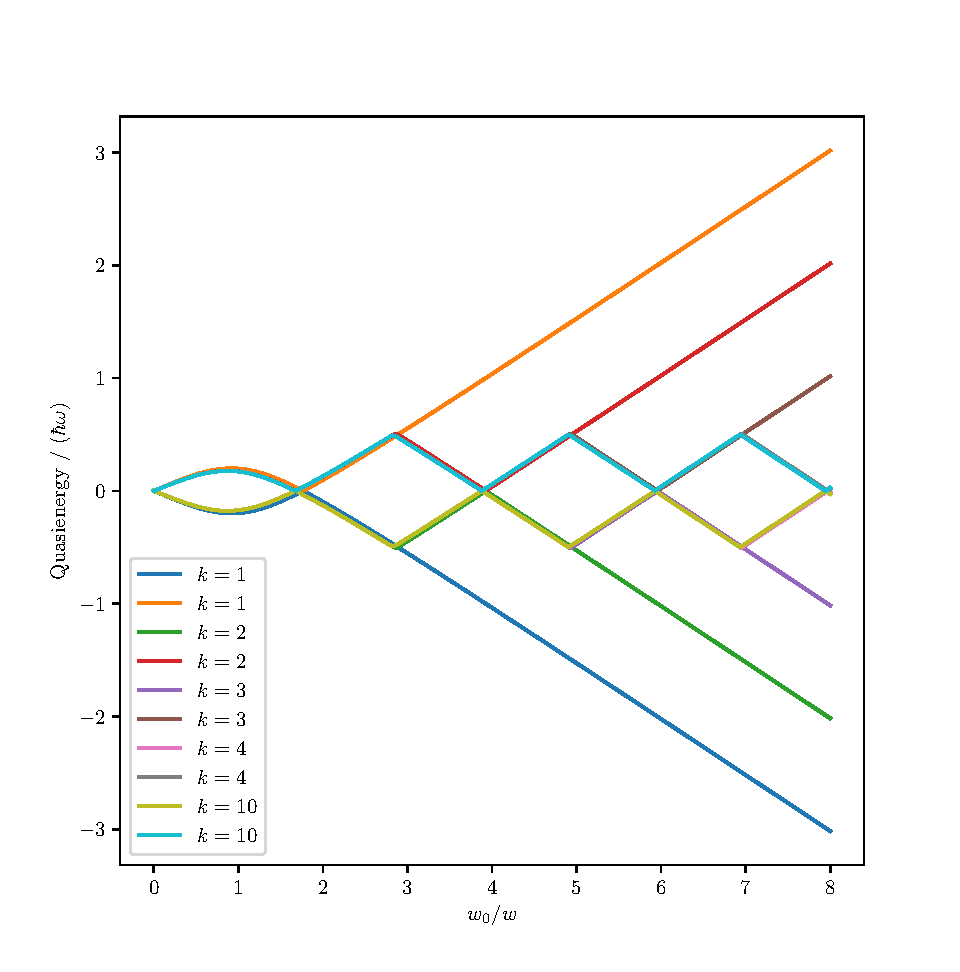
\includegraphics[width=0.6\linewidth]{q3-quasienergy.pdf}
      \caption{Quasienergies vs.\ $\omega_0$}
      \label{fig:q3-quasienergy}
    \end{figure} 
    Note that the off-diagonal coupling mixes these states, and the non-zero off-diagonal terms will directly mix the the dressed states which differ in energy by $\hbar\omega$ and 
    When $0<\omega_0/\omega\lesssim 2$, $0 < \Delta$ to make $\ket{E_1}$ mix with $\ket{E_2}$ we need only one Floquet Brillouin zone since the only the dressed $\ket{E_1}$; when $2 \lesssim \omega_0/\omega \lesssim 4$, we need 2 Floquet Brillouin zone; and so on.
    This can be seen by selecting specific submatrix to diagonalize for the whole matrix, \ie, change the truncated basis by $\set{\ket{\alpha n}}_{n=-k}^{k}$, and the results are also plotted in Figure~\ref{fig:q3-quasienergy}.
    \item The time averaged transition probability in Eq.~19 in Shirley 1965 can be written in our notations as
    \begin{align*}
      \bar{P}_{\alpha\to\beta} = \sum_{n}\sum_{\lambda} \abs{ {\ip{\beta n}{U_{\lambda}}}{\ip{U_{\lambda}}{\alpha 0}}}^2.
    \end{align*}
    This can be justified from the definition of $\bar{P}_{\alpha\to\beta}$
    \begin{align*}
      {P}_{\alpha\to\beta} &= \abs{U_{\beta\alpha}(0,\ t)}^2 = \abs{\mel{\beta}{e^{-\iu H t/\hbar}}{\alpha}}^2.
    \end{align*}
    On the other hand, note that $\bra{t}\ket{\alpha 0} = \ket{\alpha}$ for all $t$. Insert the spectrum decomposition of identity operator in the space spanned by $\set{\ket{n}}$ and we have
    \begin{align*}
      \mel{\beta}{U(0,\ t)}{\alpha} 
      =& \bra{\beta}\sum_{n}\op{n} U \bra{t}\ket{\alpha 0}
      =  \sum_{n} \ip{t}{n} \bra{\beta n} U\ket{\alpha 0}
      = \sum_{n} e^{\iu n\omega t} \bra{\beta n} \sum_\lambda\ket{U_\lambda}e^{-\iu\mathcal{E}_\lambda t/\hbar}\bra{U_\lambda} \ket{\alpha 0}.
    \end{align*}
    Therefore,
    \begin{align*}
      {P}_{\alpha\to\beta} &= \abs{\sum_{n}\sum_\lambda e^{\iu (n\omega - \mathcal{E}_\lambda/\hbar)t} \bra{\beta n}\ket{U_\lambda}\bra{U_\lambda} \ket{\alpha 0}}^2
    \end{align*}
    If we take the time average, then contributions of the crossing phases are zeros, and the diagonal phases are ones. Hence
    \begin{align*}
      \bar{P}_{\alpha\to\beta} = \sum_{n}\sum_{\lambda} \abs{ {\ip{\beta n}{U_{\lambda}}}{\ip{U_{\lambda}}{\alpha 0}}}^2.
    \end{align*}

    \item See Figure~\ref{fig:q3-transition}. Here the size of the truncated basis $k$ is 10 and has been verified consistency with the case that $k=100$. 
    \begin{figure}[H]
      \centering
      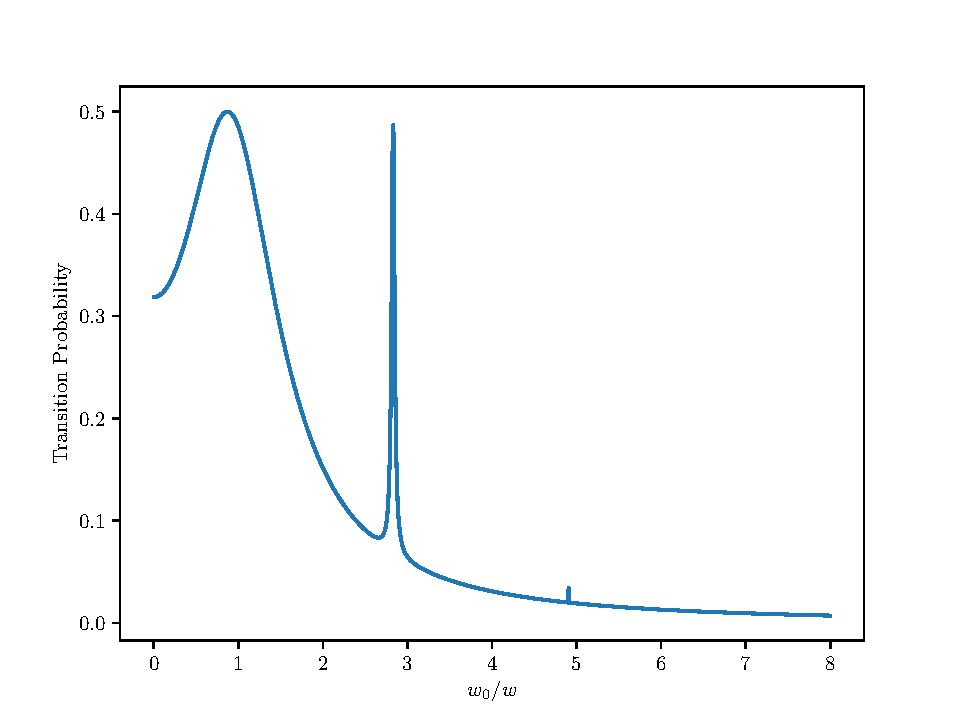
\includegraphics[width=0.6\linewidth]{q3-transition.pdf}
      \caption{Transition probability vs.\ $\omega_0$}
      \label{fig:q3-transition}
    \end{figure}
    \item 
    It is clear that there are peaks in Figure~\ref{fig:q3-transition} at $\omega_0/\omega \approx 1,\ 3,\ 5$, and the peaks are almost invisible as $\omega_0/\omega$ gets larger.
    This this because when $\omega_0/\omega$ is nearly odd, the system is more likely to absorb correct amount of energy in laser and then the transition happens, while when $\omega_0/\omega$ is nearly even, since the Floquet modes shares almost the same energy, it is not that likely to absorb correct amount of energy in laser.
  \end{enumerate}

  \item
  \begin{enumerate}[(i)]
    \item Let $\set{\ket{n}}_{n=1}^{\infty}$ be an orthonormal and complete basis. Then 
    \begin{align*}
      \tr(\hat{A}\hat{B}) =& \sum_n \ev{\hat{A}\hat{B}}{n} = \sum_n \bra{n}\hat{A}\sum_m\ket{m}\bra{m}\hat{B}\ket{n} = \sum_n \sum_m \mel{n}{\hat{A}}{m} \mel{m}{\hat{B}}{n} \\
      =& \sum_m \sum_n \mel{m}{\hat{B}}{n} \mel{n}{\hat{A}}{m} = \sum_m \ev{\hat{B}\hat{A}}{m} = \tr(\hat{B}\hat{A});
    \end{align*}
    and
    \begin{align*}
      \ev{\hat{A}} = \ev{\hat{A}}{\Psi} = \bra{\Psi}\hat{A}\sum_n \ket{n}\bra{n}\ket{\Psi} 
      = \sum_n \bra{\Psi}\hat{A}\ket{n}\bra{n}\ket{\Psi} =\sum_n \bra{n}\ket{\Psi} \bra{\Psi}\hat{A}\ket{n} = \sum_n \bra{n}\hat{\rho}\hat{A}\ket{n} = \tr(\hat{\rho} \hat{A}).
    \end{align*}
    \item For $\ket{E_1}$:
    \begin{align*}
      \rho_1 = \mqty(1 & 0)^\dagger\mqty(1 & 0) = \mqty(
        1 & 0 \\ 0 & 0
      );
    \end{align*}
    for $\ket{E_2}$:
    \begin{align*}
      \rho_2 = \mqty(0 & 1)^\dagger\mqty(0 & 1) = \mqty(
        0 & 0 \\ 0 & 1
      );
    \end{align*}
    for $(\ket{E_1} + \iu\ket{E_2})/\sqrt{2}$:
    \begin{align*}
      \rho_3 = \frac{1}{2} \mqty(1 \\ \iu)\mqty(1 & -\iu) = \frac{1}{2}\mqty(
        1 & -\iu \\ \iu & 1
      );
    \end{align*}
    for a mixture with $P_1$ to be in $\ket{E_1}$ and $P_2$ to be in $(\ket{E_1} + \iu\ket{E_2})/\sqrt{2}$:
    \begin{align*}
      \rho_4 = P_1 \rho_1 + P_2 \rho_3 = \mqty(
        P_1 + P_2/2 & -\iu P_2/2 \\ \iu P_2/2 & P_2/2
      );
    \end{align*}
    \item Consider a two-level system $\rho = \sum_n P_n \op{\phi_n}$, where $\ket{\phi_n} = c_{n1}\ket{E_1} + c_{n2}\ket{E_2}$ is normalized, and $\ket{E_1}$ and $\ket{E_2}$ construct an orthonormal basis of the Hilbert space, $P_n$ is the (positive) possibility of finding the system in $\ket{\phi_n}$. It is clear that $\rho$ is hermite since $\rho^\dagger = \sum_n P_n^* \op{\phi_n} = \sum_n P_n \op{\phi_n} = \rho$. 
    And hence, we can diagonalize $\rho$ such that
    \begin{align*}
      \rho = w_1\op{\psi_1} + w_2\op{\psi_2},
    \end{align*}
    where $w_1$ and $w_2$ are nonnegative, and$\set{\ket{\psi_1},\ \ket{\psi_2}}$ spans the same Hilbert space as $\set{\ket{E_1},\ \ket{E_2}}$, and is orthonormal. Note that 
    \begin{align*}
      \tr\rho = w_1 + w_2 = 1,
    \end{align*}
    and therefore, $\rho^2 = w_1^2\op{\psi_1} + w_2^2\op{\psi_2}$
    \begin{align*}
      \tr\rho^2 = w_1^2 + w_2^2 = w_1^2 + (1-w_1)^2 = 2 w_1^2 - 2w_1 + 1.
    \end{align*}
    Since $0 \leq w_1 \leq 1$, therefore, $1/2  \leq \tr\rho^2 \leq 1$.
    Note that when $w_1 = w_2 = 1/2$, $\tr \rho^2$ gets its minimal $1/2$ and when $w_1 = 0$ or $w_1 = 1$, $\tr\rho^2$ gets its maximal $1$.
    
    The entropy of such a two-level system is
    \begin{align*}
      S =& - \tr(\rho \ln\rho) = - \tr((w_1\op{\psi_1} + w_2\op{\psi_2})(\ln w_1 \op{\psi_1} + \ln w_2 \op{\psi_2}))
      \\ =& - \tr(w_1\ln w_1 \op{\psi_1} + w_2\ln w_2 \op{\psi_2}) = - w_1\ln w_1 - w_2\ln w_2 = - w_1\ln w_1 - (1-w_1)\ln (1-w_1),
    \end{align*}
    where $0 \leq w_1 \leq 1$. Note that when $w_1 = w_2 = 1/2$, $S$ gets its maximal $\ln 2$ and when $w_1 = 0$ or $w_1 = 1$, $\tr\rho^2$ gets its minimal $0$.
    
    We can relate the two quantities by defining the R\'enyi entropy
    \begin{align*}
      R_\alpha = \frac{1}{1-\alpha}\ln \tr\rho^\alpha,
    \end{align*}
    and notice that
    \begin{align*}
      R_2 = \frac{1}{1-2}\ln \tr\rho^2 = -\ln \tr\rho^2,
    \end{align*}
    and
    \begin{align*}
      R_1 = \lim_{\alpha \to 1} \frac{1}{1-\alpha}\ln \tr\rho^\alpha = - \lim_{\alpha \to 1} \frac{ \tr \rho^{\alpha}\ln \rho}{\tr \rho^\alpha} = - \frac{ \tr \rho\ln\rho}{\tr \rho} = -  \tr \rho\ln\rho= S.
    \end{align*}
    \item The entropy is not time independent: consider a spin--boson model (SBM) stating with the initial state $\qty(\ket{E_1} + \ket{E_2})/\sqrt{2}\otimes\ket{0}$, where $\ket{0}$ is at the ground state of the harmonic oscillator. The numerical simulation gives Figure~\ref{fig:q4-ce}.
    \begin{figure}[H]
      \centering
      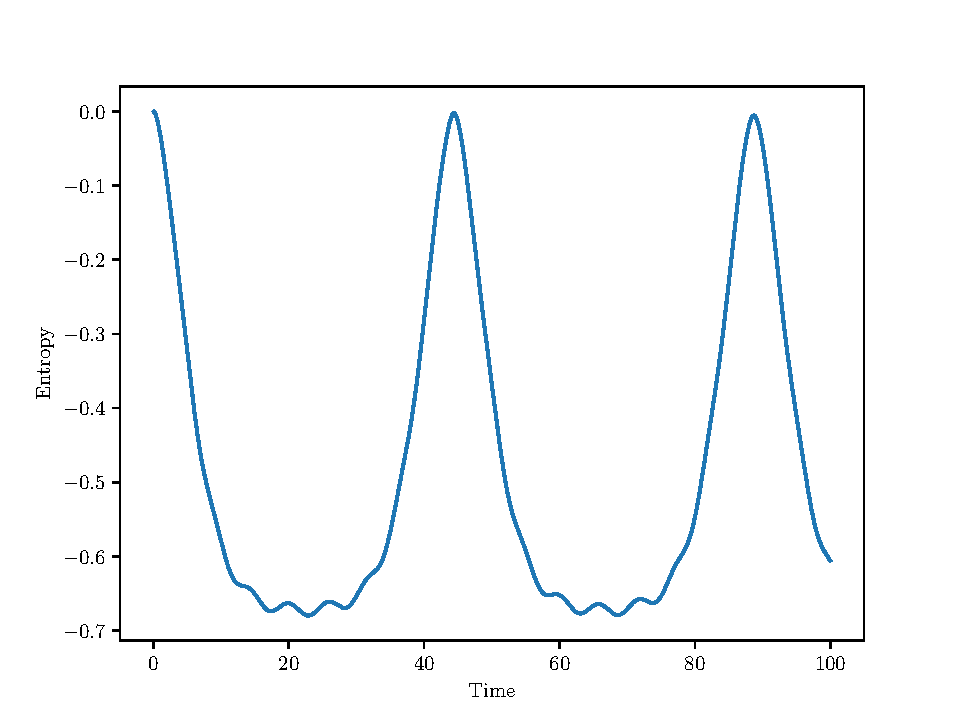
\includegraphics[width=0.6\linewidth]{q4-ce.pdf}
      \caption{Time-dependency of entropy for spin--boson model.}
      \label{fig:q4-ce}
    \end{figure}
  \end{enumerate}

  \item
  \begin{enumerate}[(i)]
    \item Recall the definition of $A_\mathrm{W}(q,\ p) = \int_{-\infty}^{\infty}\dd{y}\mel{q-y/2}{\hat{A}(\hat{q},\ \hat{p})}{q + y/2} e^{\iu p y / \hbar}$. Therefore, 
    \begin{align*}
      q_\mathrm{W} =& \int_{-\infty}^{\infty}\dd{y}\mel{q-y/2}{\hat{q}}{q + y/2} e^{\iu p y / \hbar}
      \\
      =& \int_{-\infty}^{\infty}\dd{y} \int_{-\infty}^{\infty} \dd{x} \delta(x - q + y/2) (q+y/2) \delta(x - q - y/2) e^{\iu p y / \hbar} \\
      =& \int_{-\infty}^{\infty}\dd{y} (q+y/2)\delta(y) e^{\iu p y / \hbar}
      = qe^{\iu p \cdot 0 / \hbar} = q,
    \end{align*}
    and similarly,
    \begin{align*}
      p_\mathrm{W} =& \int_{-\infty}^{\infty}\dd{y}\mel{q-y/2}{\hat{p}}{q + y/2} e^{\iu p y / \hbar}
      \\
      =& \int_{-\infty}^{\infty}\dd{y} \int_{-\infty}^{\infty} \dd{x} \delta(x - q + y/2) \iu\hbar\pdv{x} \delta(x - q - y/2) e^{\iu p y / \hbar} \\
      =& \iu\hbar\int_{-\infty}^{\infty}\dd{y} \int_{-\infty}^{\infty} \dd{x} \delta(x - q + y/2) \delta'(x - q - y/2) e^{\iu p y / \hbar}\\
      =& \iu\hbar\int_{-\infty}^{\infty}\dd{y}\delta'(- y)  e^{\iu p y / \hbar} 
      = -\iu\hbar\int_{-\infty}^{\infty}\dd{y}\delta'(y)  e^{\iu p y / \hbar} \\
      =& -\iu\hbar\eval{\qty(e^{\iu p y / \hbar})'}_{y = 0} = p.
    \end{align*}
    \begin{lemma}
      For any operators $\hat{A}(\hat{q},\ \hat{p})$ and $\hat{B}(\hat{q},\ \hat{p})$, $aA_\mathrm{W} + bB_\mathrm{W} = \qty(a{A} + b{B})_W$, where $a,\ b$ are any complex numbers.
    \end{lemma}
    \begin{proof}
      Note that
      \begin{align*}
        A_\mathrm{W} =& \int_{-\infty}^{\infty}\dd{y}\mel{q-y/2}{\hat{A}}{q + y/2} e^{\iu p y / \hbar},
        \\
        B_\mathrm{W} =& \int_{-\infty}^{\infty}\dd{y}\mel{q-y/2}{\hat{B}}{q + y/2} e^{\iu p y / \hbar},
        \\
        (aA+bB)_\mathrm{W} =& \int_{-\infty}^{\infty}\dd{y}\mel{q-y/2}{{aA+bB}}{q + y/2} e^{\iu p y / \hbar}\\
        =& \int_{-\infty}^{\infty}\dd{y}\qty(a\mel{q-y/2}{\hat{A}}{q + y/2} + b\mel{q-y/2}{\hat{B}}{q + y/2})e^{\iu p y / \hbar}\\
        =& a\int_{-\infty}^{\infty}\dd{y}\mel{q-y/2}{\hat{A}}{q + y/2} e^{\iu p y / \hbar} + b\int_{-\infty}^{\infty}\dd{y}\mel{q-y/2}{\hat{B}}{q + y/2} e^{\iu p y / \hbar} \\
        =& aA_\mathrm{W} + bB_\mathrm{W}.
      \end{align*}
    \end{proof}
    \begin{lemma}
      $\qty(\hat{q}^n)_\mathrm{W} = q^n$, $\qty(\hat{p}^n)_\mathrm{W} = p^n$.
    \end{lemma}
    \begin{proof}
      \begin{align*}
        \qty(\hat{q}^n)_\mathrm{W}  =& \int_{-\infty}^{\infty}\dd{y}\mel{q-y/2}{\hat{q}^n}{q + y/2} e^{\iu p y / \hbar}
        \\
        =& \int_{-\infty}^{\infty}\dd{y} \int_{-\infty}^{\infty} \dd{x} \delta(x - q + y/2) (q+y/2)^n \delta(x - q - y/2) e^{\iu p y / \hbar} \\
        =& \int_{-\infty}^{\infty}\dd{y} (q+y/2)^n\delta(y) e^{\iu p y / \hbar}
        = q^n,
      \end{align*}
      and
      \begin{align*}
        \qty(\hat{p}^n)_\mathrm{W} =& \int_{-\infty}^{\infty}\dd{y}\mel{q-y/2}{\hat{p}^n}{q + y/2} e^{\iu p y / \hbar}
        \\
        =& \int_{-\infty}^{\infty}\dd{y} \int_{-\infty}^{\infty} \dd{x} \delta(x - q + y/2) (\iu\hbar)^n\pdv[n]{x} \delta(x - q - y/2) e^{\iu p y / \hbar} \\
        =& (\iu\hbar)^n\int_{-\infty}^{\infty}\dd{y} \int_{-\infty}^{\infty} \dd{x} \delta(x - q + y/2) \delta^{(n)}(x - q - y/2) e^{\iu p y / \hbar}\\
        =& (\iu\hbar)^n\int_{-\infty}^{\infty}\dd{y}\delta^{(n)}(- y)  e^{\iu p y / \hbar} 
        = (-\iu\hbar)^n\int_{-\infty}^{\infty}\dd{y}\delta^{(n)}(y)  e^{\iu p y / \hbar} \\
        =& (-\iu\hbar)^n\eval{\qty(e^{\iu p y / \hbar})^{(n)}}_{y = 0} = p^n.
      \end{align*}
    \end{proof}
    Therefore, if $\hat{T}$ and $\hat{W}$ converge to their Taylor series, then
    \begin{align*}
      H_\mathrm{W} =& (T(p) + V(q))_\mathrm{W} = \qty(\sum_{n=0}^{\infty} \frac{1}{n!}\dv[n]{T}{p}p^n + \sum_{n=0}^{\infty} \frac{1}{n!}\dv[n]{V}{q}q^n)_\mathrm{W}\\
      =& \sum_{n=0}^{\infty} \frac{1}{n!}\dv[n]{T}{p}p_\mathrm{W}^n + \sum_{n=0}^{\infty} \frac{1}{n!}\dv[n]{V}{q}q_\mathrm{W}^n
      =\sum_{n=0}^{\infty} \frac{1}{n!}\dv[n]{T}{p}p^n + \sum_{n=0}^{\infty} \frac{1}{n!}\dv[n]{V}{q}q^n
      =T(p)+ V(q) = H(q,\ p).
    \end{align*}

    \item For a pure state, $\hat{\rho} = \op{\psi}$, and
    \begin{align*}
      \rho_\mathrm{W} =& \frac{1}{2\pi\hbar}\int_{-\infty}^{\infty} \dd{y} \mel{q-y/2}{\hat{\rho}}{q + y/2}e^{\iu p y / \hbar} \\
      =&\frac{1}{2\pi\hbar}\int_{-\infty}^{\infty} \dd{y} \psi(q+y/2)^*\psi(q-y/2)e^{\iu p y / \hbar},
    \end{align*}
    Then
    \begin{align*}
      \lim_{\hbar \to 0}\rho_\mathrm{W} =& \frac{1}{2\pi\hbar}\int_{-\infty}^{\infty} \dd{y} \mel{q-y/2}{\hat{\rho}}{q + y/2}e^{\iu p y / \hbar} \\
      =&\frac{1}{2\pi}\int_{-\infty}^{\infty} \dd{y} \psi(q+y/2)^*\psi(q-y/2)\lim_{\hbar \to 0}e^{\iu p y / \hbar}/\hbar,
    \end{align*}
    and note that $e^{\iu p y / \hbar}$ oscillates when $\hbar \to +0$. Therefore, $\rho_\mathrm{W}$ is singular for a pure quantum state.
    
    \item We need the following lemma.
    \begin{lemma}
      For any operator $\hat{A}(\hat{q},\ \hat{p})$, $(A^\dagger)_\mathrm{W} = \qty({A_\mathrm{W}})^*$.
    \end{lemma}
    \begin{proof}
      Note that
      \begin{align*}
        (A^\dagger)_\mathrm{W} =& \int_{-\infty}^{\infty}\dd{y}\mel{q-y/2}{\hat{A}^{\dagger}}{q + y/2} e^{\iu p y / \hbar}
        \\
        =& \int_{-\infty}^{\infty}\dd{y}\mel{q+y/2}{\hat{A}}{q - y/2}^* e^{\iu p y / \hbar}\\
        =& \int_{-\infty}^{\infty}\dd{y}\mel{q-y/2}{\hat{A}}{q + y/2}^* e^{-\iu p y / \hbar}\\
        =& \qty({A_\mathrm{W}})^*
      \end{align*}
    \end{proof}
    \begin{align*}
      \dv{\qty(\hat{O}_H)_\mathrm{W}}{t} =& \qty(-\frac{\iu}{\hbar}\comm{\hat{O}_H}{\hat{H}_H})_\mathrm{W}\\
      =& -\frac{\iu}{\hbar}((\hat{O}_H\hat{H}_H)_\mathrm{W}-(\hat{H}_H\hat{O}_H)_\mathrm{W})\\
      =& -\frac{\iu}{\hbar}((\hat{O}_H\hat{H}_H)_\mathrm{W}-((\hat{O}_H\hat{H}_H)_\mathrm{W})^*).
    \end{align*}
    Recall that $\qty(\hat{A}\hat{B})_\mathrm{W} = A_\mathrm{W} e^{-\frac{\iu\hbar}{2}\tensor{\Lambda}}B_\mathrm{W}$, where $\tensor{\Lambda} = \overleftarrow{\pdv{p}}\overleftarrow{\pdv{q}} - \overrightarrow{\pdv{q}}\overrightarrow{\pdv{p}}$, therefore,
    \begin{align*}
      \dv{\qty(\hat{O}_H)_\mathrm{W}}{t} 
      =& -\frac{\iu}{\hbar}((\hat{O}_H)_\mathrm{W} e^{-\frac{\iu\hbar}{2}\tensor{\Lambda}} (\hat{H}_H)_\mathrm{W} - \qty((\hat{O}_H)_\mathrm{W} e^{-\frac{\iu\hbar}{2}\tensor{\Lambda}} (\hat{H}_H)_\mathrm{W})^*) \\
      =& -\frac{\iu}{\hbar}((\hat{O}_H)_\mathrm{W} e^{-\frac{\iu\hbar}{2}\tensor{\Lambda}} (\hat{H}_H)_\mathrm{W} - (\hat{O}_H)_\mathrm{W}^* e^{\frac{\iu\hbar}{2}\tensor{\Lambda}} (\hat{H}_H)_\mathrm{W}^*)\\
      =& -\frac{2}{\hbar}(\hat{O}_H)_\mathrm{W} \sin{\frac{\hbar\tensor{\Lambda}}{2}} (\hat{H}_H)_\mathrm{W}.
    \end{align*}
    In the last step we have applied the fact that $(\hat{O}_H)_\mathrm{W}$ is real for any
    Hermitian $\hat{O}_H$ since $(\hat{O}_H)_\mathrm{W} = (\hat{O}_H^\dagger)_\mathrm{W} = ((\hat{O}_H)_\mathrm{W})^*$.
    \item When $\hbar \to 0$, $(\hat{O}_H)_\mathrm{W} = O^c + \hbar O_1 + o(\hbar)$, $(\hat{H}_H)_\mathrm{W} = H^c + \hbar H_1 + o(\hbar)$, and $\sin {\frac{\hbar\tensor{\Lambda}}{2}} = \frac{\hbar\tensor{\Lambda}}{2} + o(\hbar)$, then,
    \begin{align*}
     & \dv{\qty(\hat{O}_H)_\mathrm{W}}{t} = -\frac{2}{\hbar}(\hat{O}_H)_\mathrm{W} \sin{\frac{\hbar\tensor{\Lambda}}{2}} (\hat{H}_H)_\mathrm{W}\\
     \Rightarrow & \dv{O^c}{t} + o(1) = -2O^c\frac{\tensor{\Lambda}}{2} H^c + o(1) \\
     \Rightarrow & \dv{O^c}{t} = \acomm{H^c}{O^c}_P + o(1),
    \end{align*} 
    where $\acomm{\cdot}{\cdot}_P$ is the Poisson bracket.
    \item When we use the wigner representation and take the limit of $\hbar \to 0$ then we recover the classical mechanics, which means that the classical mechanics is a specific representation of quantum mechanics under the limit that Planck constant is small enough.
  \end{enumerate}

  \item Code is available at \url{https://github.com/vINyLogY/QD-hw2}.
  \begin{enumerate}[(A)]
    \item
    \begin{enumerate}[(i)]
      \item Here we only need to focus on monitoring the eigenstate with $n = 100$. Therefore the dimensionality of the grid basis should be at least 101 (assume we start counting $n$ from $0$).  We choose an overkill (checked convergence by simply increasing these parameters) dimensionality $1001$ and $q_0 = 25$, and the results are showed in Figure~\ref{fig:q6a-1}.
      \begin{figure}[H]
        \centering
        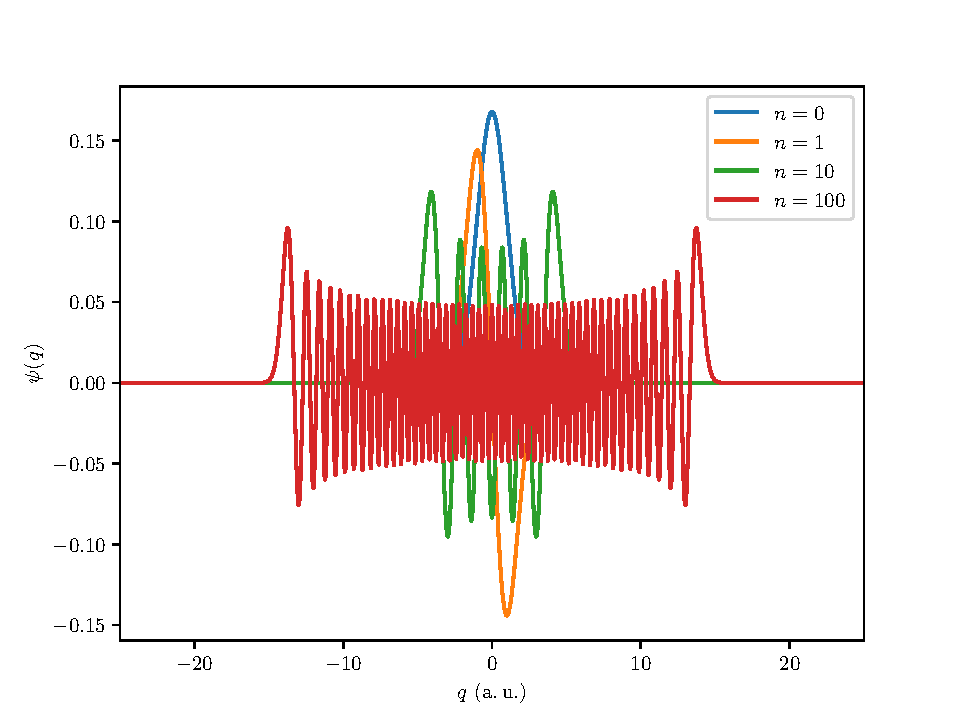
\includegraphics[width=0.6\linewidth]{q6a-1.pdf}
        \caption{$\psi(x)$ for a harmonic oscillator.}
        \label{fig:q6a-1}
      \end{figure}
      The following results are focused with $q_0 = 25$.

      \item See Figure~\ref{fig:q6a-2}.
      \begin{figure}[H]
        \centering
        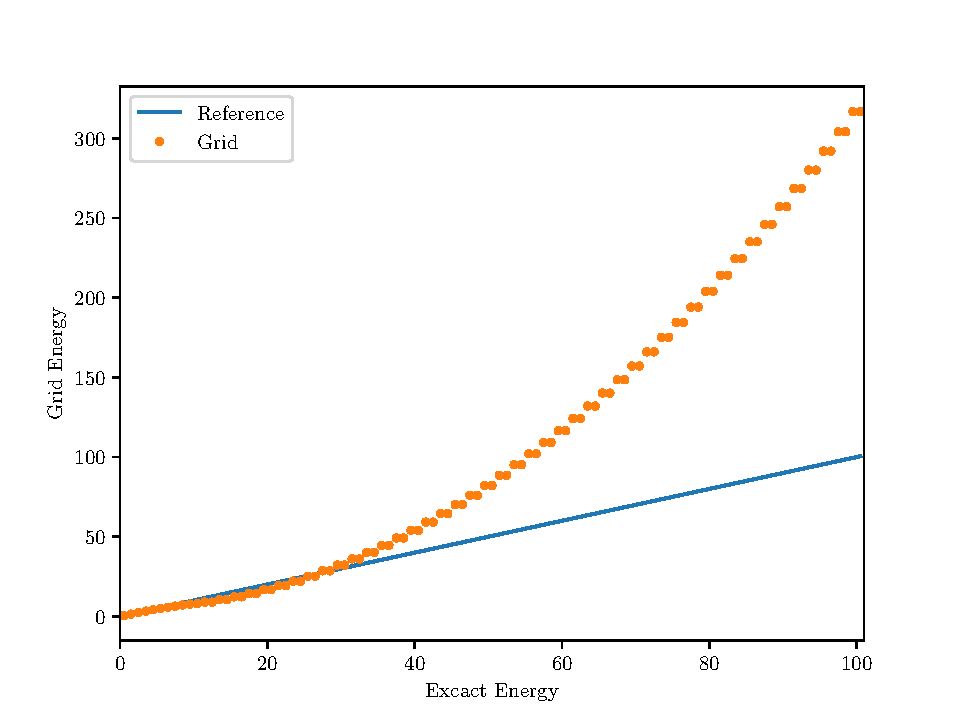
\includegraphics[width=0.6\linewidth]{q6a-2.pdf}
        \caption{Energy of each eigenstates for a harmonic oscillator.}
        \label{fig:q6a-2}
      \end{figure}
      Note that the grid method only gets the exact answer for those states with small eigenvalues. This is because for the excited states with large energy, the wavefunction oscillates crazy as showed in Figure~\ref{fig:q6a-1}, and hence we need more dense grid to characterize the wavefunction.  
      
      \item We need to change the dimensionality of grid basis in this case. For the eigenstate $n=32$, we need at least $33$ grids.
      We calculated the energy difference between the one from the grid representation and the exact one, change the dimensionality of grid basis, \ie, different $\Delta q$.
      See Figure~\ref{fig:q6a-3}.
      \begin{figure}[H]
        \centering
        \begin{minipage}{0.45\linewidth}
          \centering
          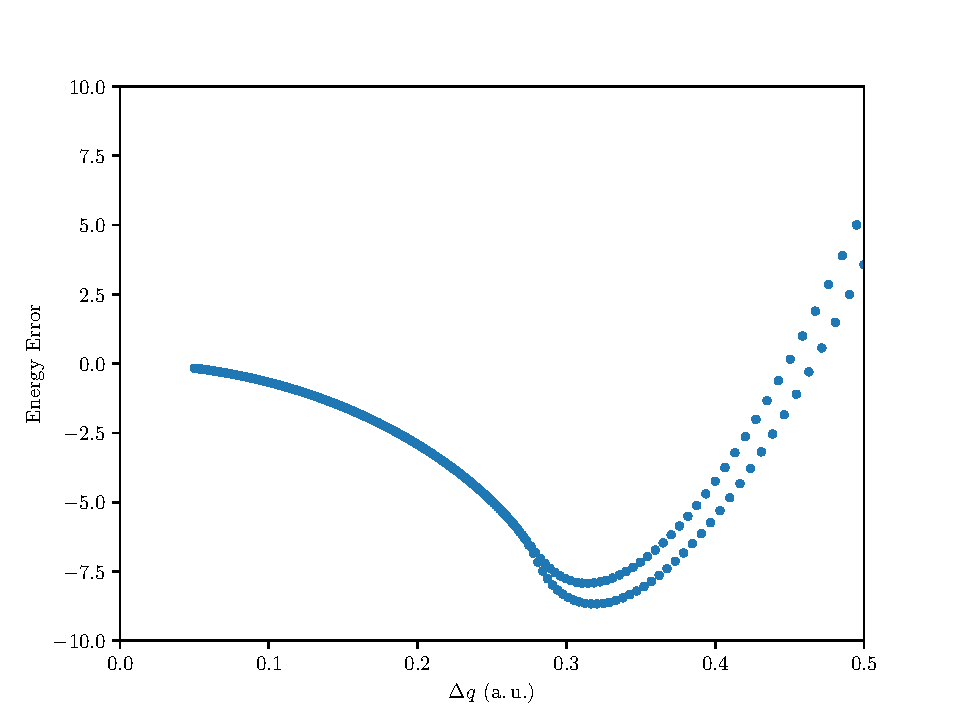
\includegraphics[width=\linewidth]{q6a-3.pdf}
        \end{minipage}
        \begin{minipage}{0.45\linewidth}
          \centering
          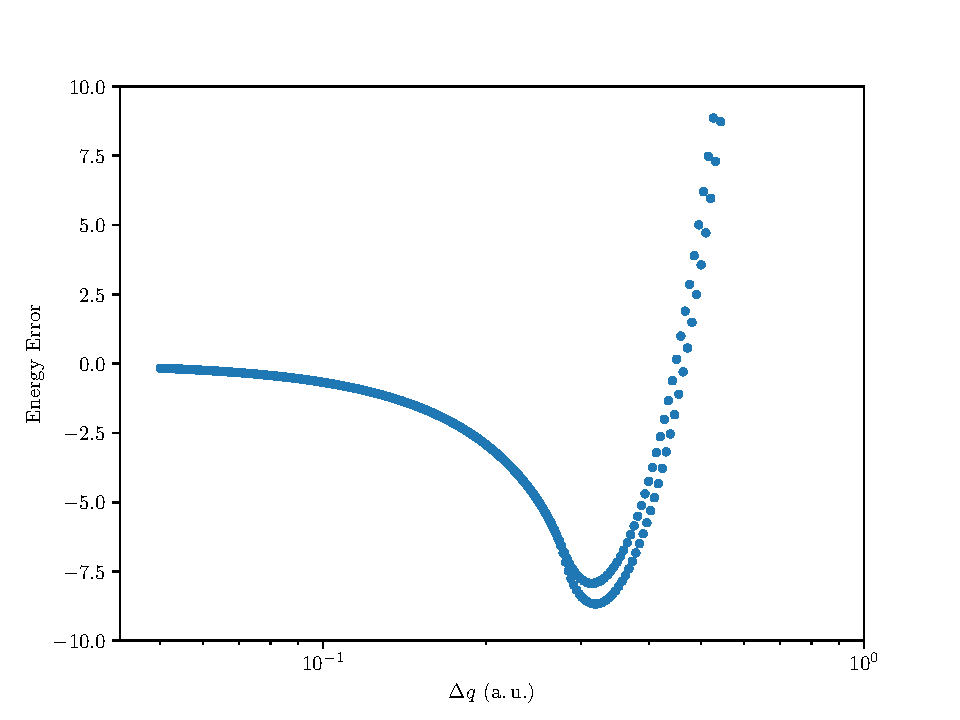
\includegraphics[width=\linewidth]{q6a-3l.pdf}
        \end{minipage}
        \caption{Energy error vs.\ $\Delta q$.}
        \label{fig:q6a-3}
      \end{figure}
    \end{enumerate}
    Therefore, $\Delta q < 0.1$ a.\,u.\ is an adequate choice.
    \item
    \begin{enumerate}[(i)]
      \item Use Sine-DVR\footnote{See \url{https://www.pci.uni-heidelberg.de/tc/usr/mctdh/lit/NumericalMethods.pdf}.} here.  
      As the concerns in grid basis, we choose the dimensionality to be 999 and $q_0 = 25$.
      See Figure~\ref{fig:q6b-1}.
      \begin{figure}[H]
        \centering
        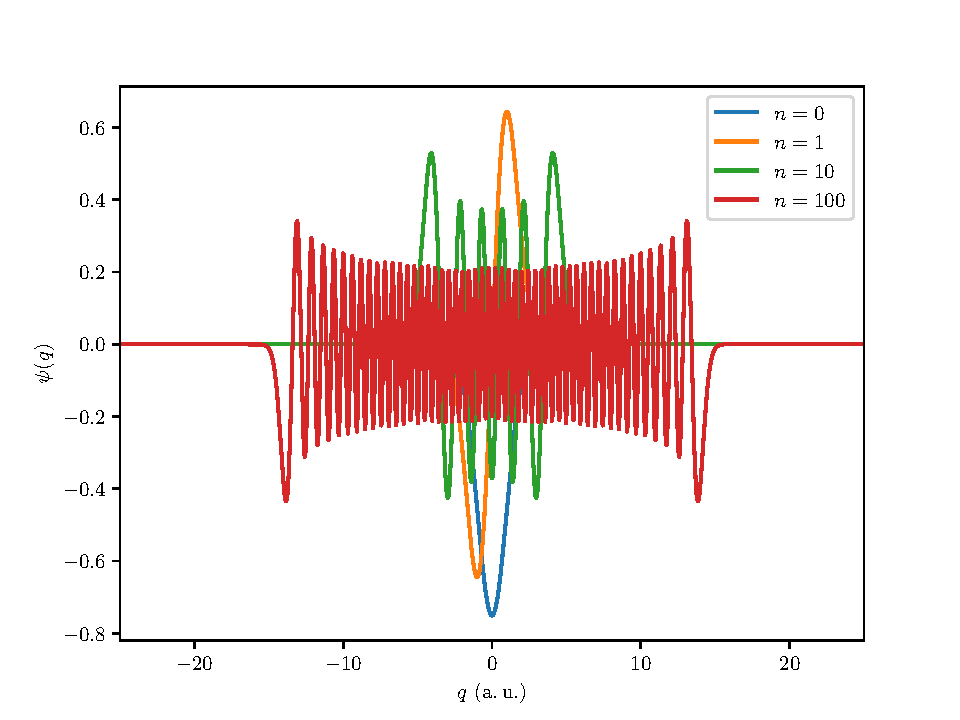
\includegraphics[width=0.6\linewidth]{q6b-1.pdf}
        \caption{Energy of each eigenstates for a harmonic oscillator.}
        \label{fig:q6b-1}
      \end{figure}
      Note that the $\psi(q)$ has up to a different phase from the results by grid basis.
      \item See Figure~\ref{fig:q6b-2}.
      \begin{figure}[H]
        \centering
        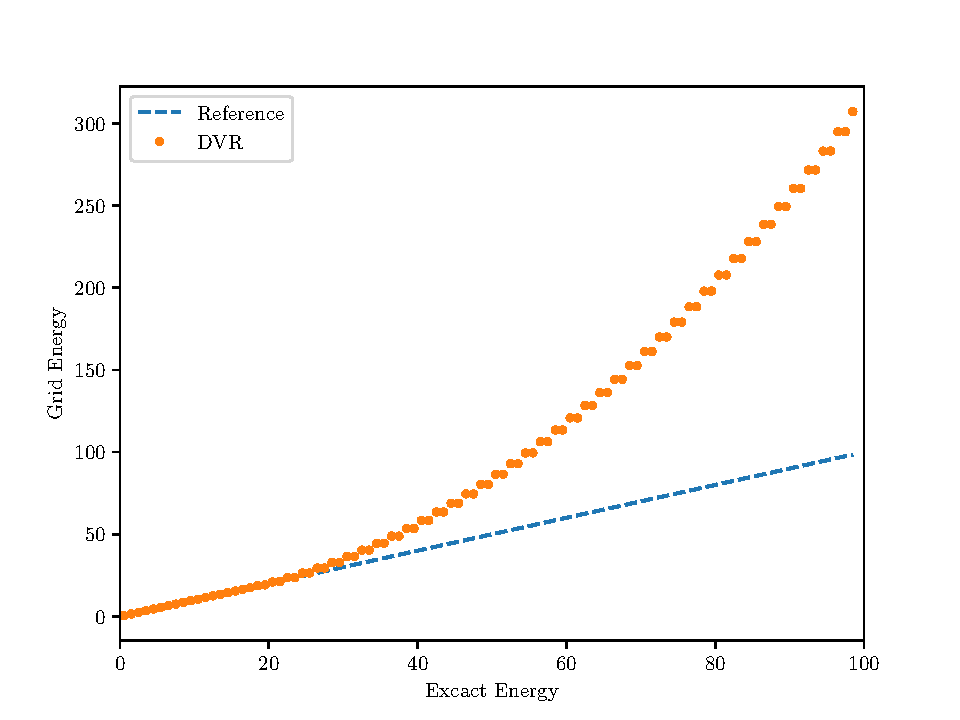
\includegraphics[width=0.6\linewidth]{q6b-2.pdf}
        \caption{Energy of each eigenstates for a harmonic oscillator.}
        \label{fig:q6b-2}
      \end{figure}
      Similarly, the DVR method only gets the exact answer for those states with small eigenvalues. This is because for the excited states with large energy, they need the basis includes the functions that corresponding to larger momentum, therefore, we need more dimensionality for the finite basis representation, or smaller grid interval, to represent such high-energy states.  

      \item We need to change the dimensionality of grid basis in this case. For the eigenstate $n=32$, we need at least $33$ grids.
      We calculated the energy difference between the one from the grid representation and the exact one, change the dimensionality of grid basis, \ie, different $\Delta q$.
      See Figure~\ref{fig:q6b-3}.
      \begin{figure}[H]
        \centering
        \begin{minipage}{0.45\linewidth}
          \centering
          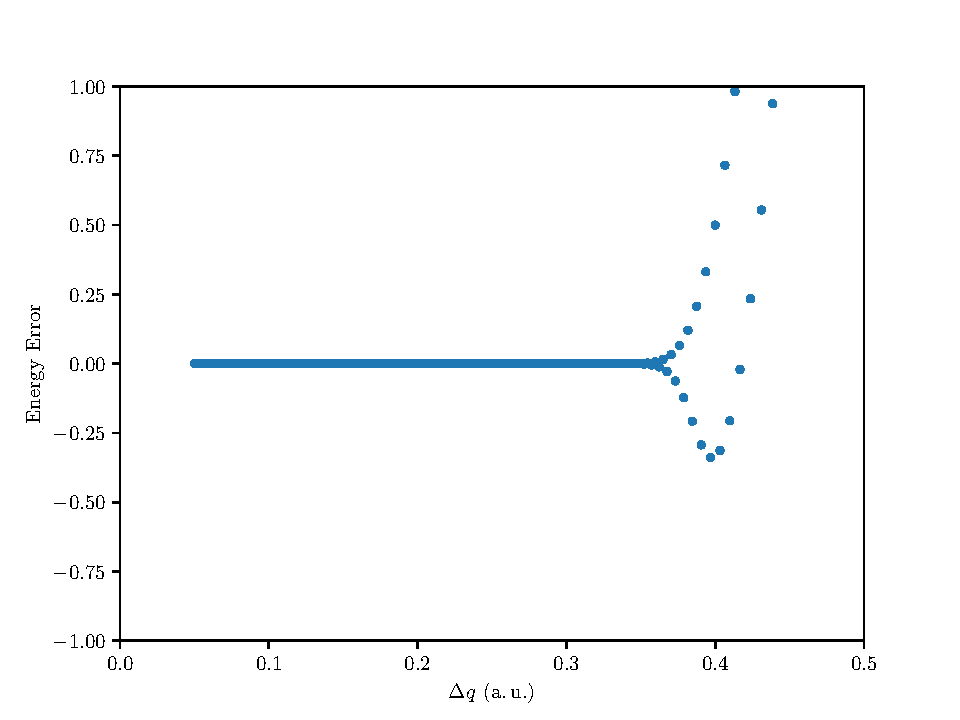
\includegraphics[width=\linewidth]{q6b-3.pdf}
        \end{minipage}
        \begin{minipage}{0.45\linewidth}
          \centering
          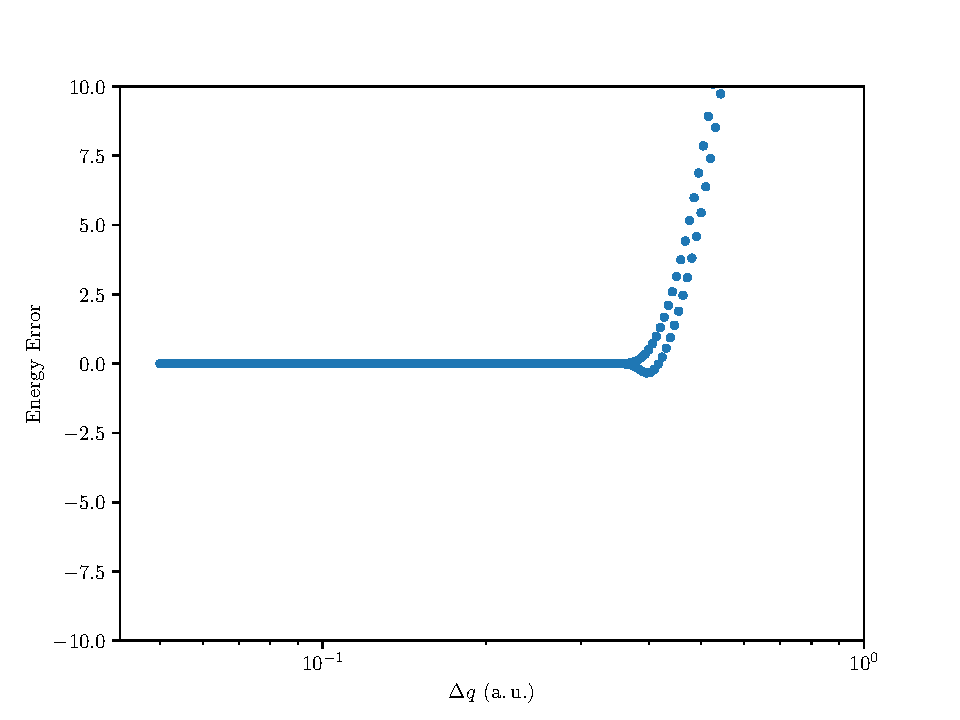
\includegraphics[width=\linewidth]{q6b-3l.pdf}
        \end{minipage}
        \caption{Energy error vs.\ $\Delta q$.}
        \label{fig:q6b-3}
      \end{figure}
      Therefore, $\Delta q < 0.1$ a.\,u.\ is an adequate choice.
      
      \item From Figure~\ref{fig:q6a-2} and Figure~\ref{fig:q6b-2} we can find that DVR can get exact energy for states with relatively larger energy when compared to grid method. Also, from Figure~\ref{fig:q6a-3} and Figure~\ref{fig:q6b-3} we can find that DVR can get exact energy with a relatively small dimensionality, or larger grid interval.
    \end{enumerate}

    \item
    \begin{enumerate}[(i)]
      \item Suppose under 1-D DVR basis $\set{\ket{\chi_i}}$ the kinetic matrix in one dimension $i$ is $T_i$, the potential matrix in one dimension $i$ is $V_i$, then the kinetic matrix of 2-D is $T_1 \otimes T_2$, and the potential matrix is a diagonal matrix $V_1 \otimes V_2$. Hence we can diagonalize the hamiltonian in the 2-D basis.
      \item See Figure~\ref{fig:q6c-2}. It is clear that for such a system, the exact eigenenergies are $E = \hbar\omega(n + 1)$, where $n = n_a + n_b$, and $n_a,\ n_b \in \mathbb{N}$. This means that for $E = \hbar\omega$, the degeneracy is 1 ($n = 0 + 0$); for $E = 2\hbar\omega$, the degeneracy is 2 ($n = 1 + 0 = 0 + 1$); for $E = 3\hbar\omega$, the degeneracy is 3 ($n = 2 + 0 = 0 + 2 = 1 + 1$); for $E = 4\hbar\omega$, the degeneracy is 4 ($n = 3 + 0 = 0 + 3 = 1 + 2 = 2 + 1$); and so on.
      From Figure~\ref{fig:q6c-2} we can also find that the parameters (upper and lower bound are both $25$ and $-25$ for each dimension; the dimensionality of basis for each degrees of freedom is 99) is sufficient for the lowest 10 eigenstates.

      \item See Figure~\ref{fig:q6c-3}.

      \begin{figure}[H]
        \centering
        \begin{minipage}{0.3\linewidth}
          \centering
          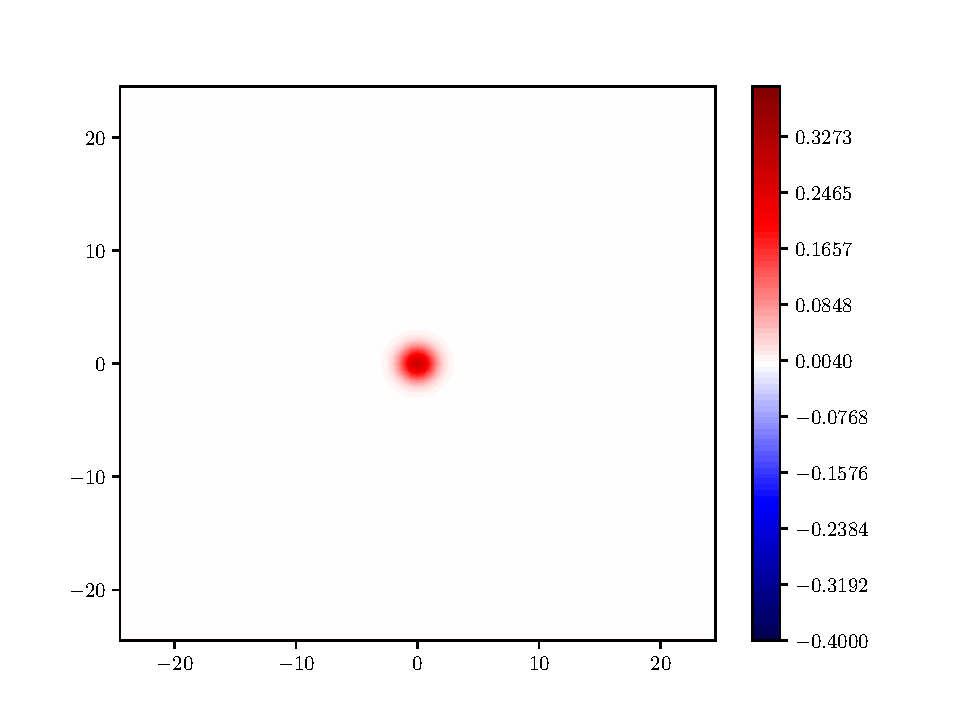
\includegraphics[width=\linewidth]{functions-0.pdf}
          \caption*{$E = 0.999999999999999889$}
        \end{minipage}
        \begin{minipage}{0.3\linewidth}
          \centering
          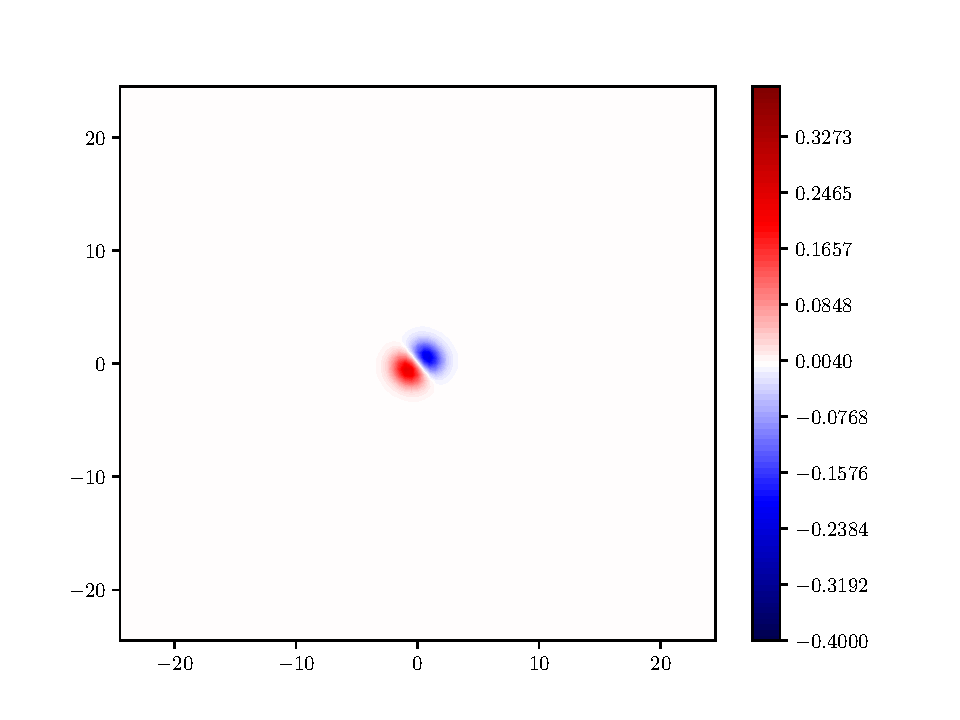
\includegraphics[width=\linewidth]{functions-1.pdf}
          \caption*{$E = 1.999999999999758860$}
        \end{minipage}
        \begin{minipage}{0.3\linewidth}
          \centering
          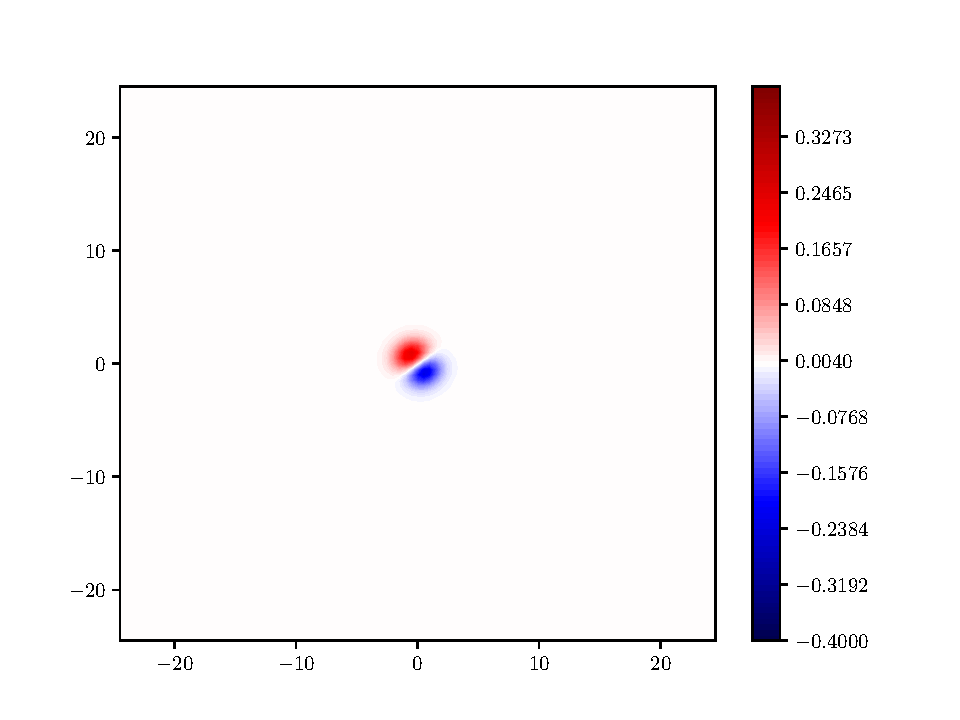
\includegraphics[width=\linewidth]{functions-2.pdf}
          \caption*{$E = 1.999999999999908962$}
        \end{minipage}

        \begin{minipage}{0.3\linewidth}
          \centering
          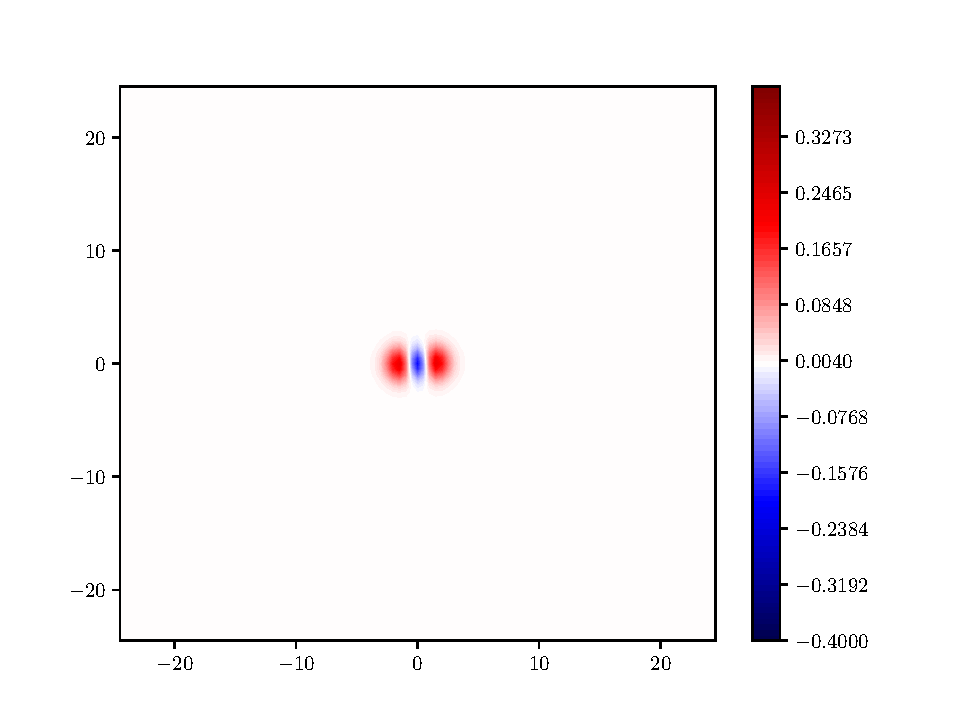
\includegraphics[width=\linewidth]{functions-3.pdf}
          \caption*{$E = 2.999999999999794387$}
        \end{minipage}
        \begin{minipage}{0.3\linewidth}
          \centering
          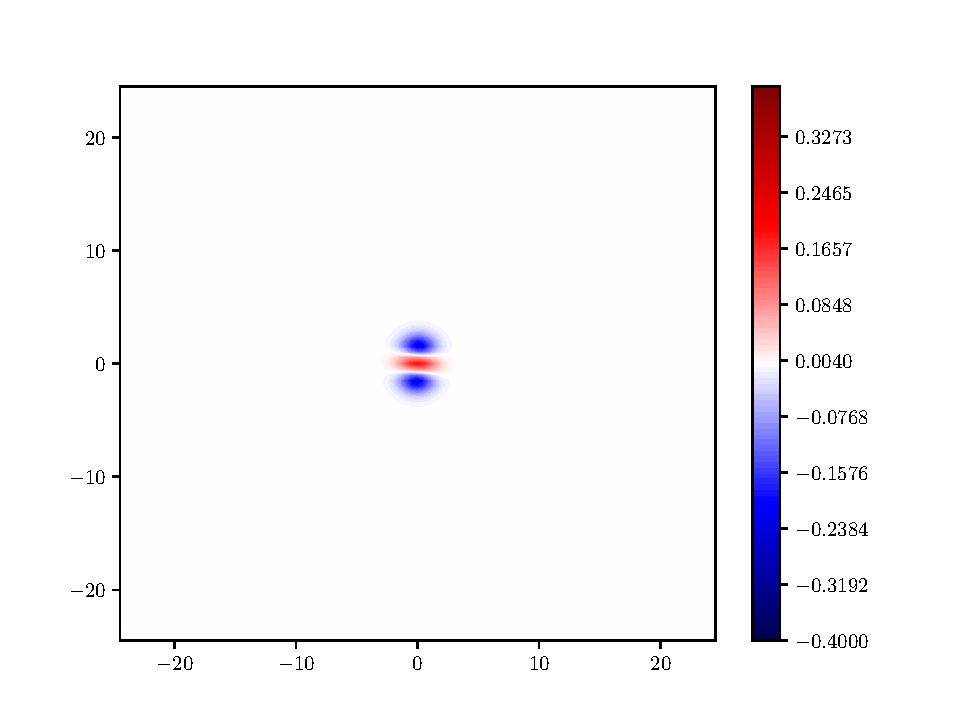
\includegraphics[width=\linewidth]{functions-4.pdf}
          \caption*{$E = 2.999999999999797939$}
        \end{minipage}
        \begin{minipage}{0.3\linewidth}
          \centering
          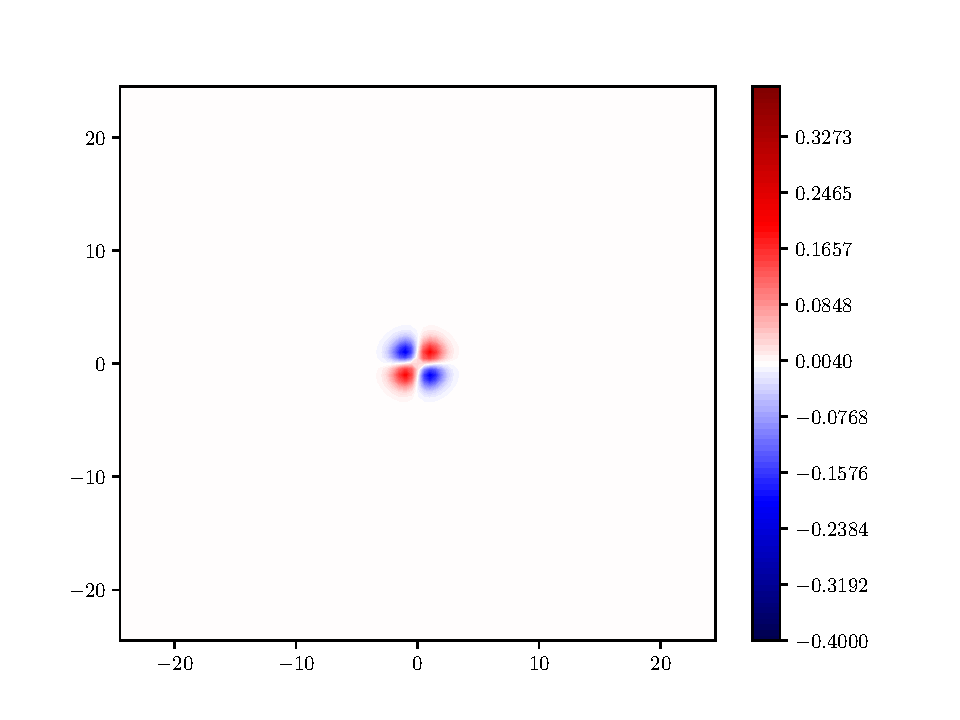
\includegraphics[width=\linewidth]{functions-5.pdf}
          \caption*{$E = 2.999999999999895195$}
        \end{minipage}

        \begin{minipage}{0.3\linewidth}
          \centering
          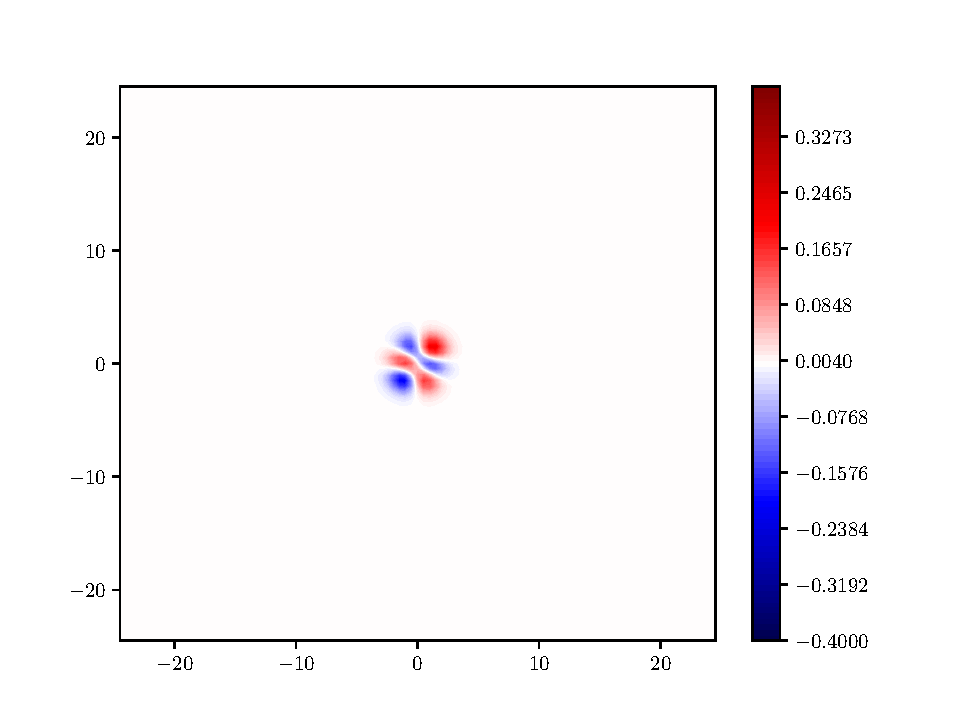
\includegraphics[width=\linewidth]{functions-6.pdf}
          \caption*{$E = 3.999999999999648281$}
        \end{minipage}
        \begin{minipage}{0.3\linewidth}
          \centering
          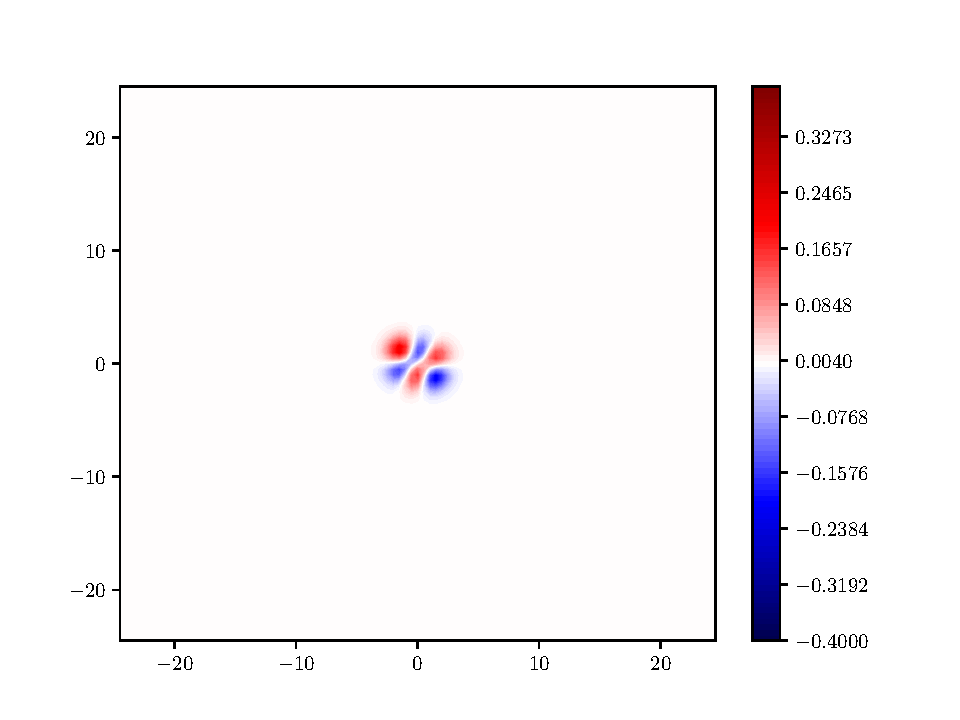
\includegraphics[width=\linewidth]{functions-7.pdf}
          \caption*{$E = 3.999999999999723332$}
        \end{minipage}
        \begin{minipage}{0.3\linewidth}
          \centering
          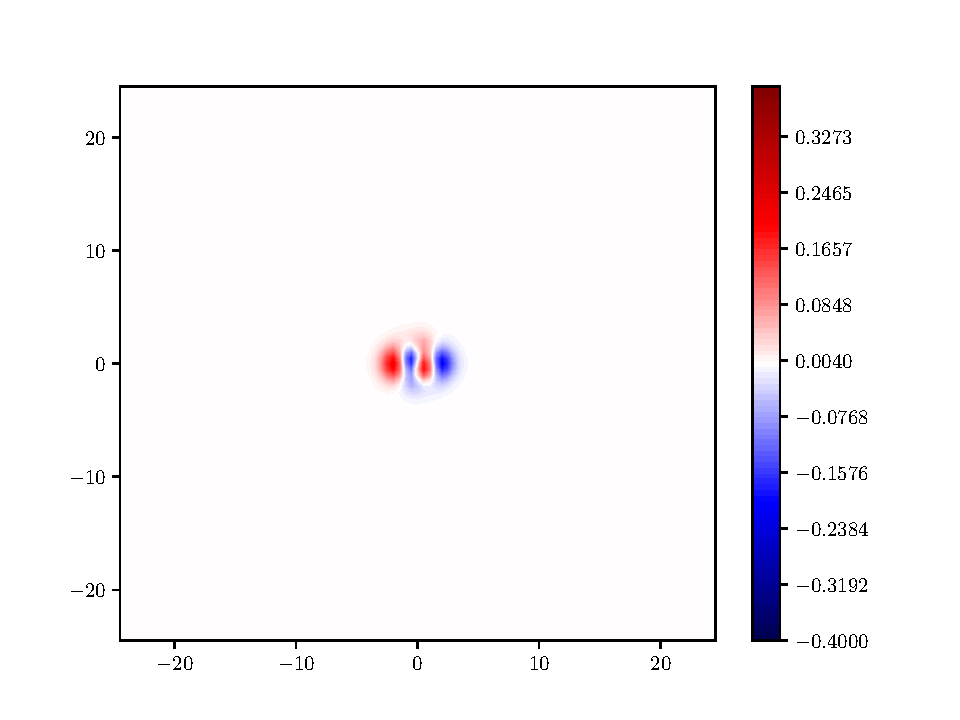
\includegraphics[width=\linewidth]{functions-8.pdf}
          \caption*{$E = 4.000000000003303136$}
        \end{minipage}

        \begin{minipage}{0.3\linewidth}
          \centering
          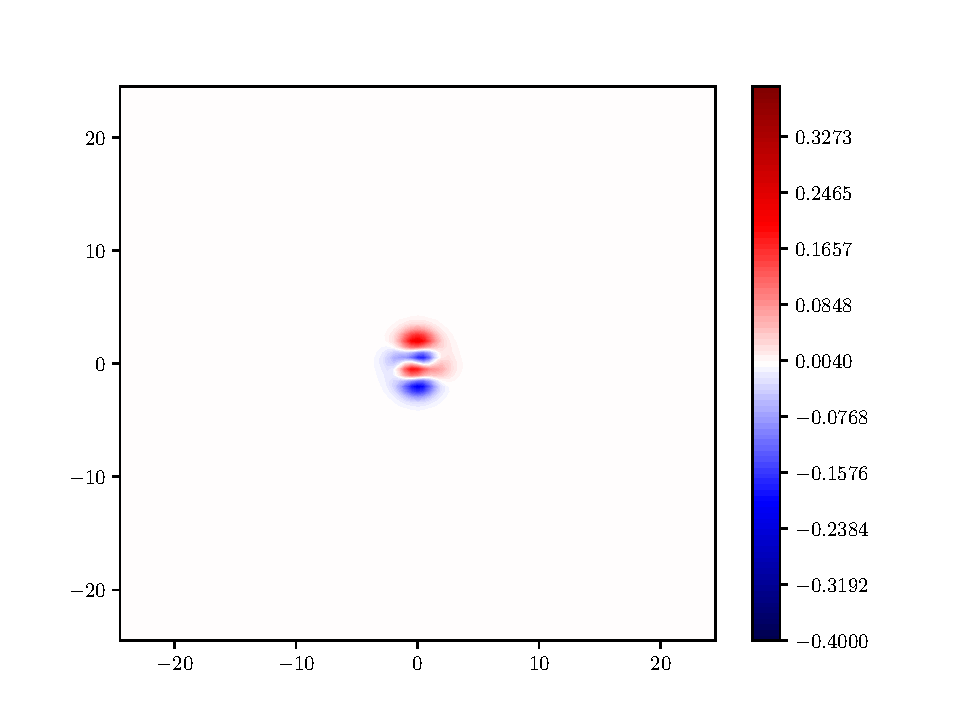
\includegraphics[width=\linewidth]{functions-9.pdf}
          \caption*{$E = 4.000000000003453238$}
        \end{minipage}
        \caption{Eigenstates and their eigenenergies for a 2-D harmonic oscillator.}
        \label{fig:q6c-2}
      \end{figure}

      \begin{figure}[H]
        \centering
        \begin{minipage}{0.3\linewidth}
          \centering
          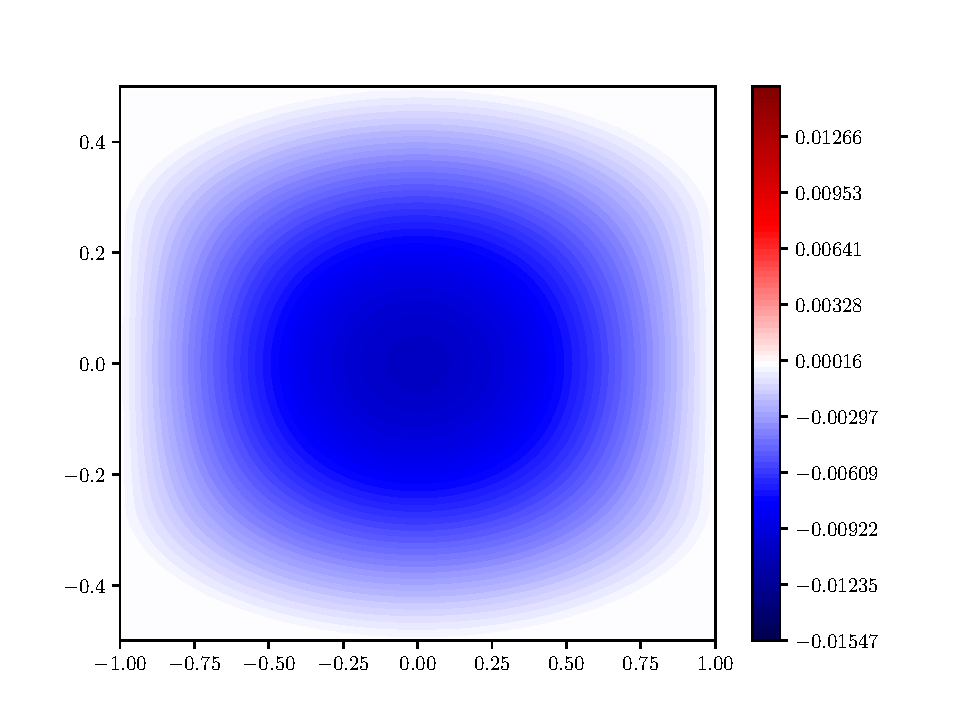
\includegraphics[width=\linewidth]{q6c-0.pdf}
          \caption*{$E_0= 6.369778636492784$}
        \end{minipage}
        \begin{minipage}{0.3\linewidth}
          \centering
          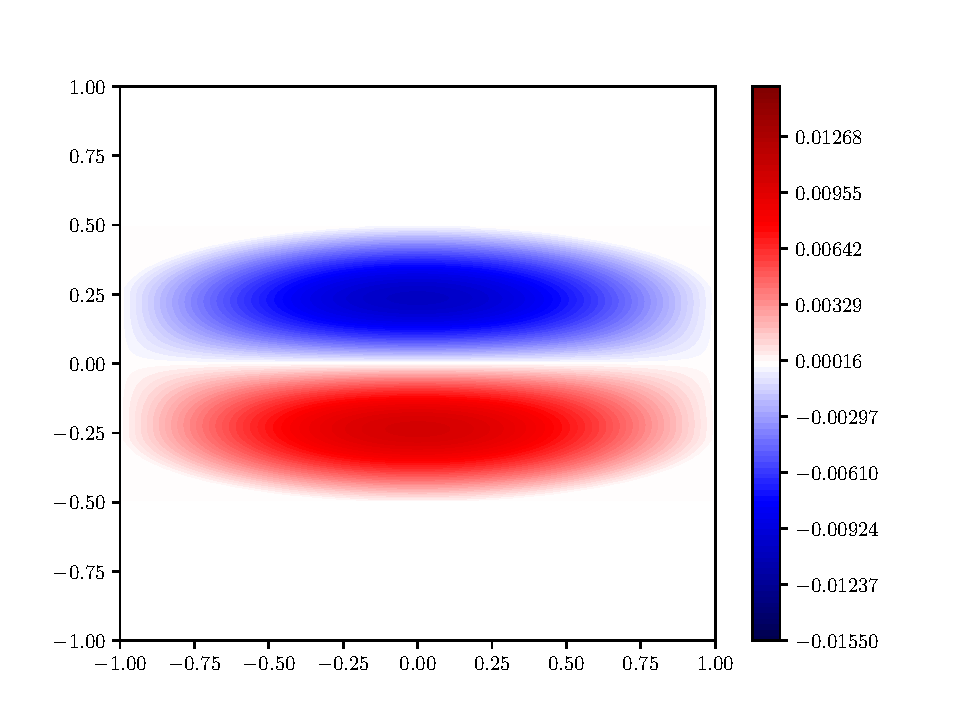
\includegraphics[width=\linewidth]{q6c-1.pdf}
          \caption*{$E_1= 10.604723421874684$}
        \end{minipage}
        \begin{minipage}{0.3\linewidth}
          \centering
          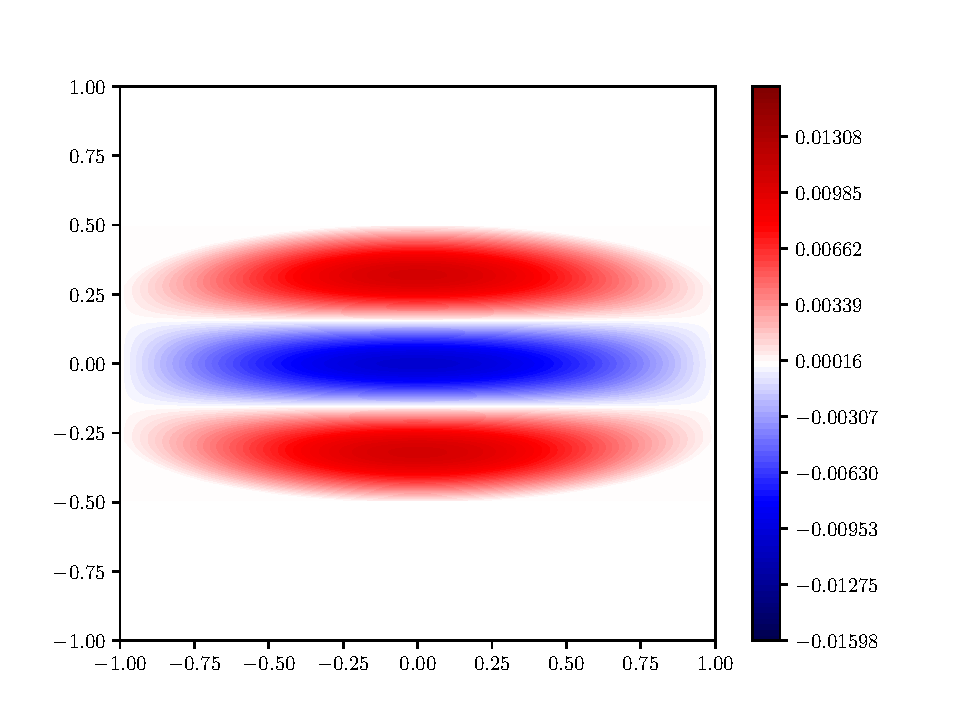
\includegraphics[width=\linewidth]{q6c-2.pdf}
          \caption*{$E_2= 17.49625007137572$}
        \end{minipage}

        \begin{minipage}{0.3\linewidth}
          \centering
          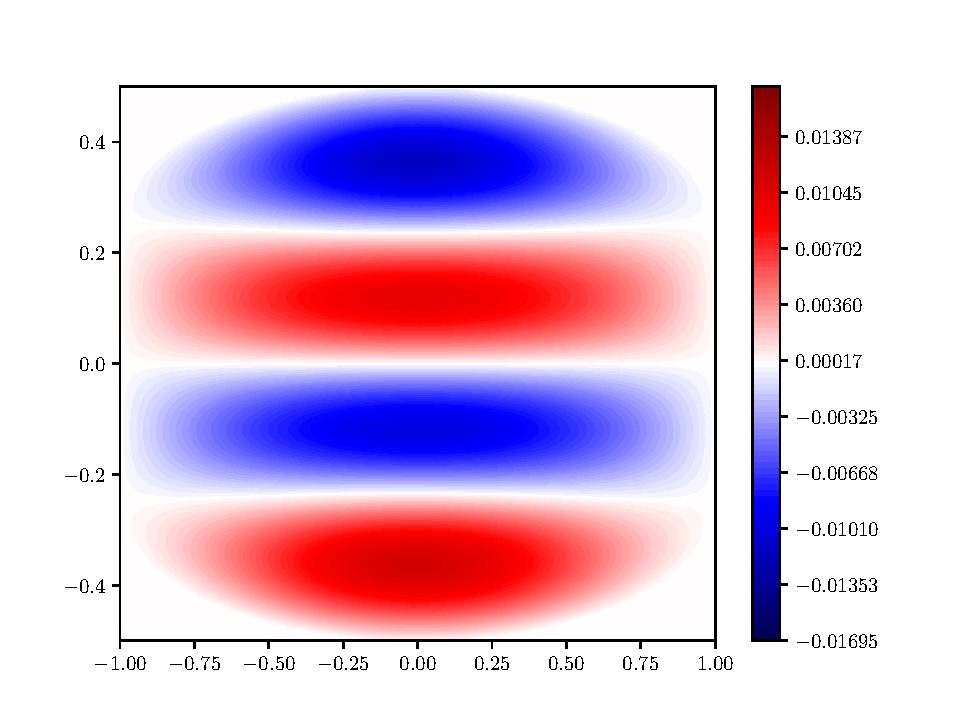
\includegraphics[width=\linewidth]{q6c-5.pdf}
          \caption*{$E_5= 26.818961595179772$}
        \end{minipage}
        \begin{minipage}{0.3\linewidth}
          \centering
          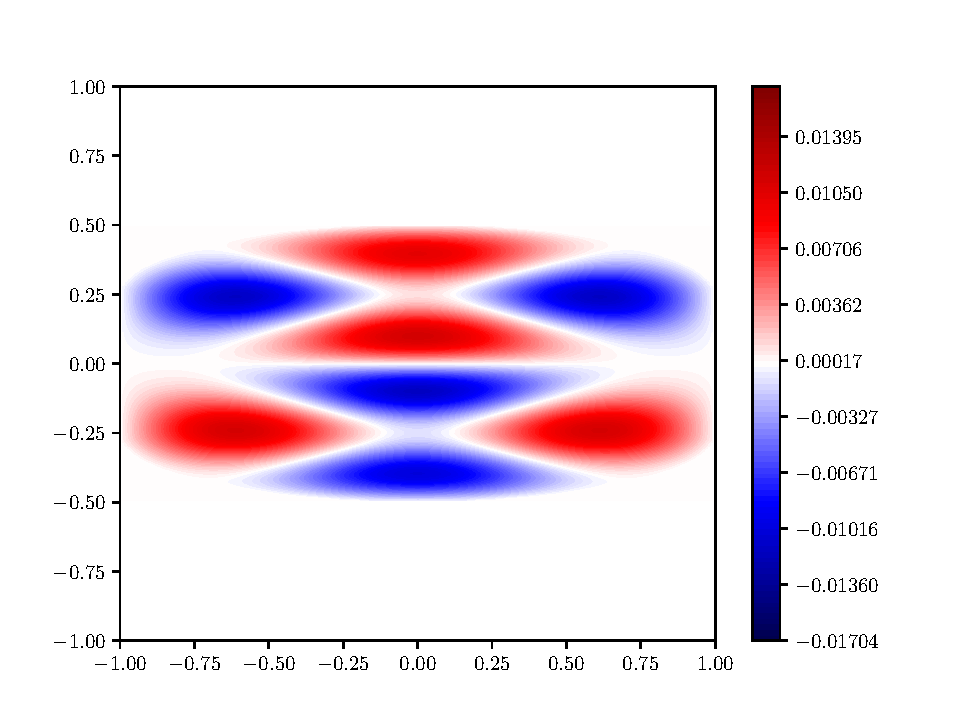
\includegraphics[width=\linewidth]{q6c-10.pdf}
          \caption*{$E_{10}= 50.75276012770485$}
        \end{minipage}
        \begin{minipage}{0.3\linewidth}
          \centering
          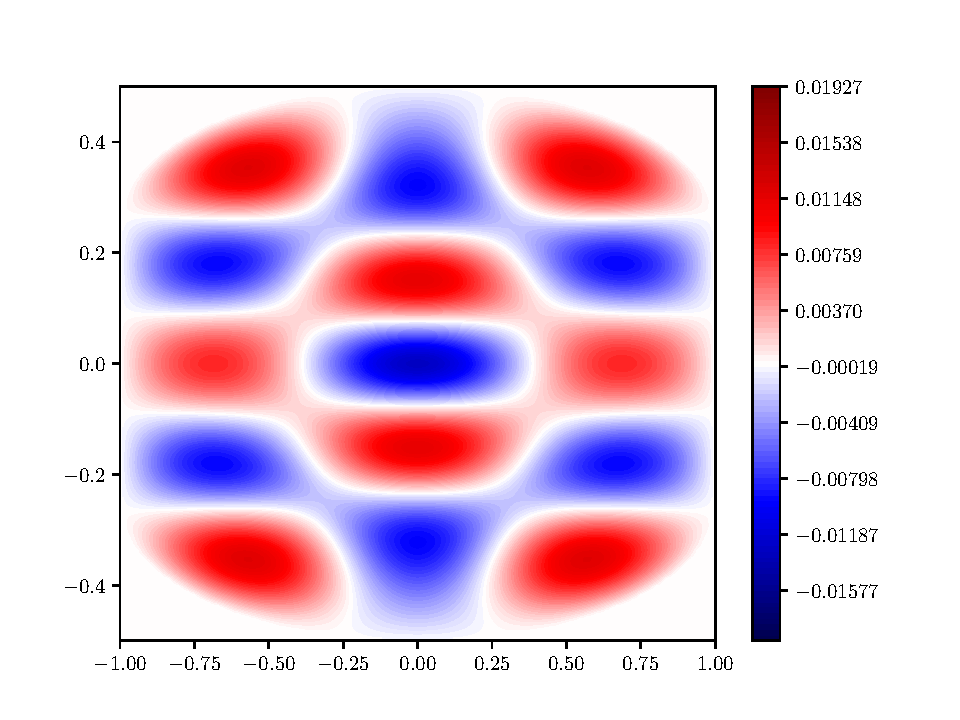
\includegraphics[width=\linewidth]{q6c-20.pdf}
          \caption*{$E_{20}= 87.88823005740137$}
        \end{minipage}

        \begin{minipage}{0.3\linewidth}
          \centering
          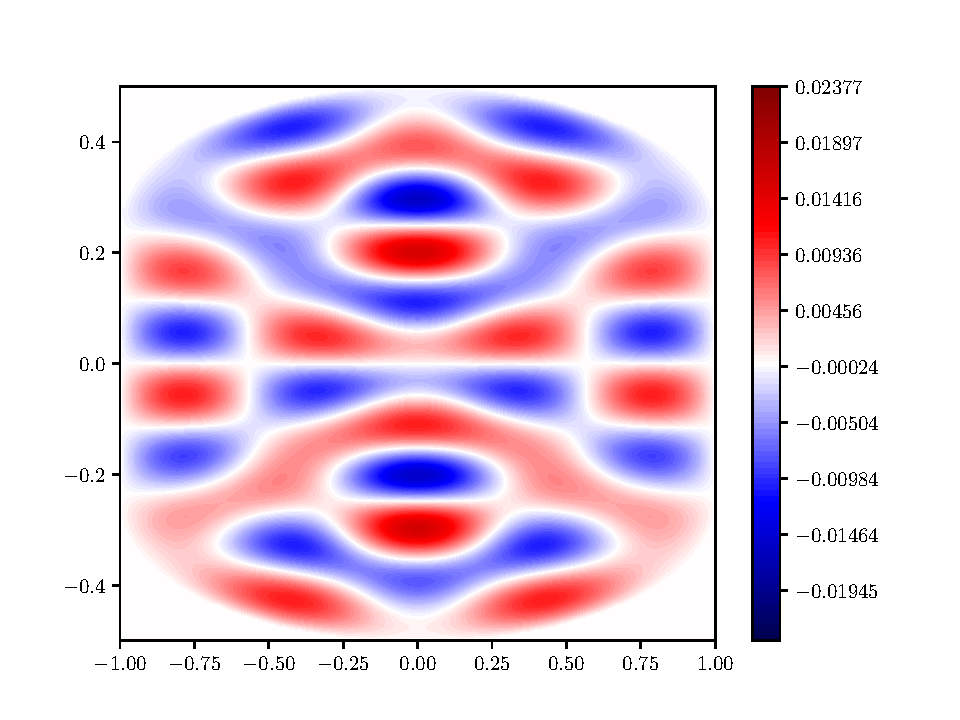
\includegraphics[width=\linewidth]{q6c-50.pdf}
          \caption*{$E_{50}= 204.00943730722977$}
        \end{minipage}
        \begin{minipage}{0.3\linewidth}
          \centering
          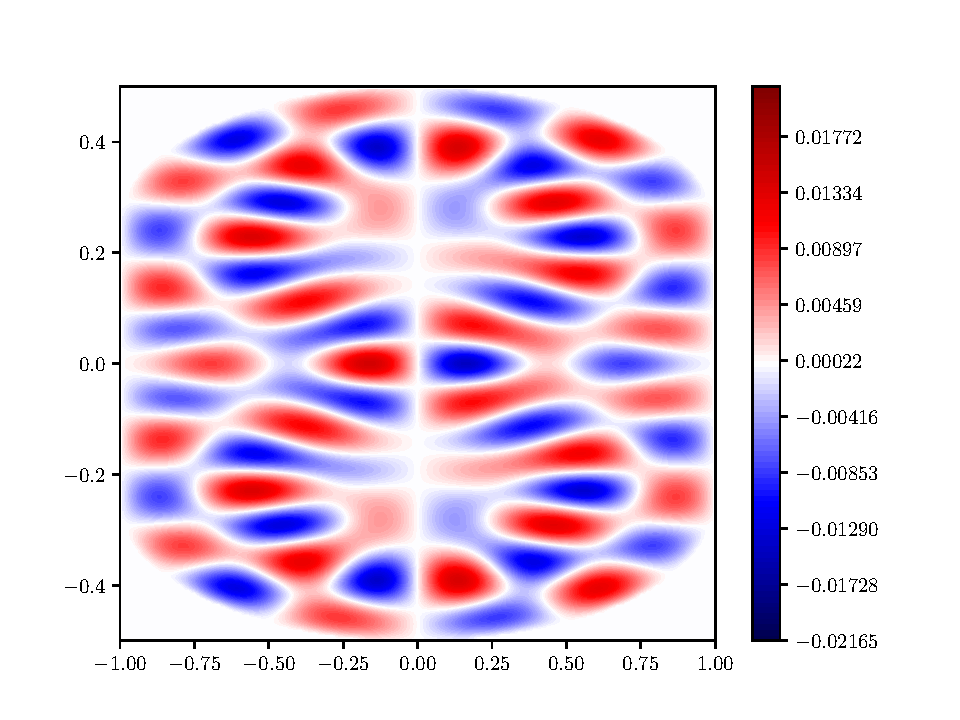
\includegraphics[width=\linewidth]{q6c-100.pdf}
          \caption*{$E_{100}= 394.4271319580347$}
        \end{minipage}
        \begin{minipage}{0.3\linewidth}
          \centering
          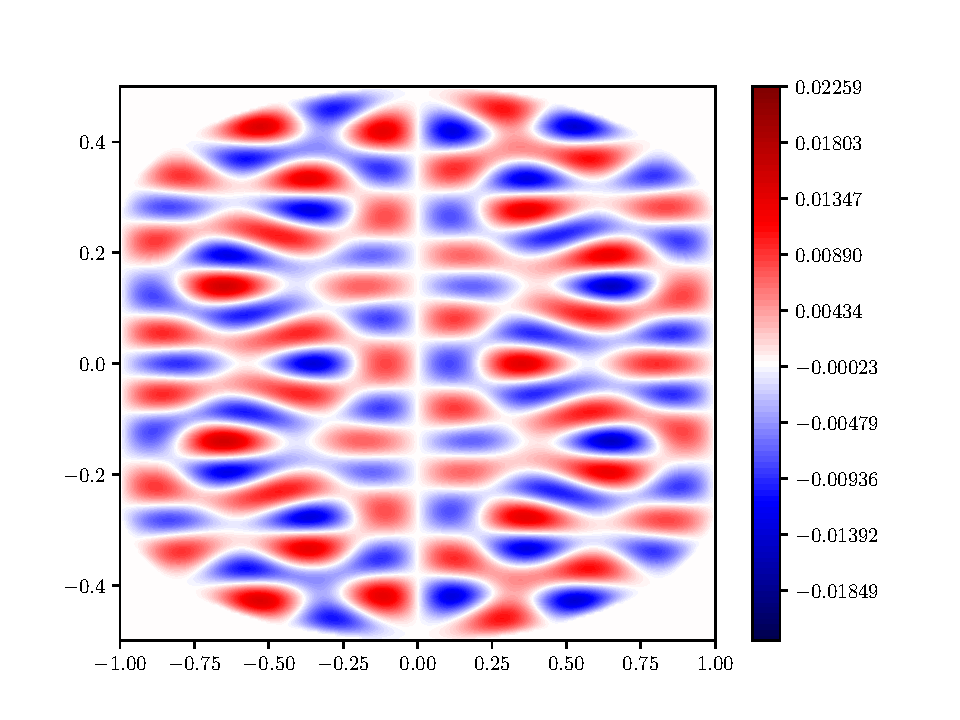
\includegraphics[width=\linewidth]{q6c-150.pdf}
          \caption*{$E_{150}= 578.41848374364$}
        \end{minipage}

        \begin{minipage}{0.3\linewidth}
          \centering
          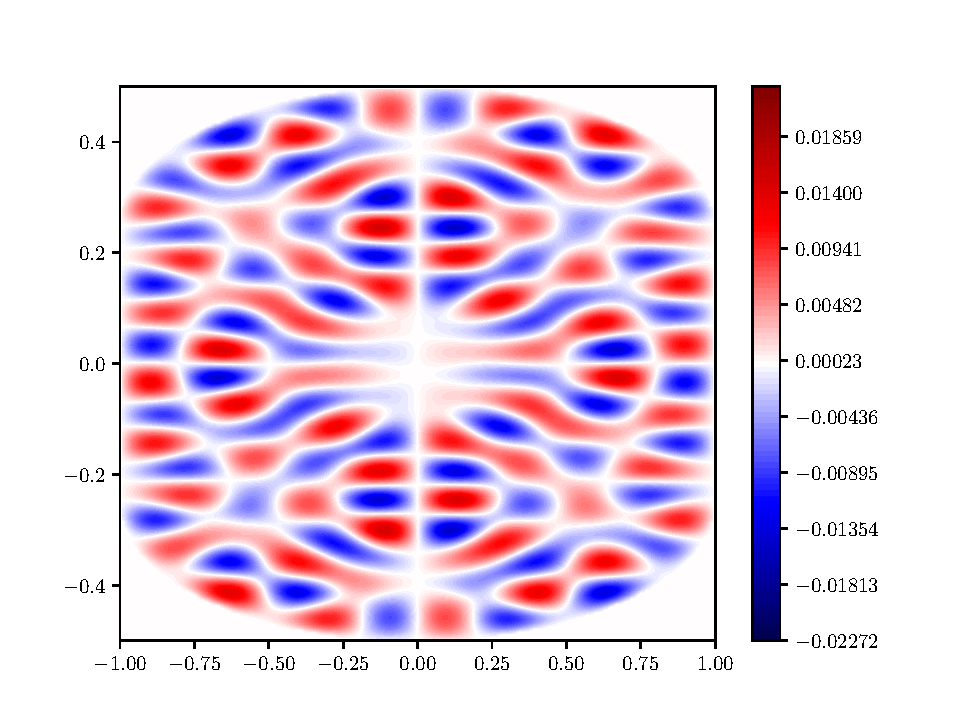
\includegraphics[width=\linewidth]{q6c-195.pdf}
          \caption*{$E_{195} = 735.5352784543273$}
        \end{minipage}
        \begin{minipage}{0.3\linewidth}
          \centering
          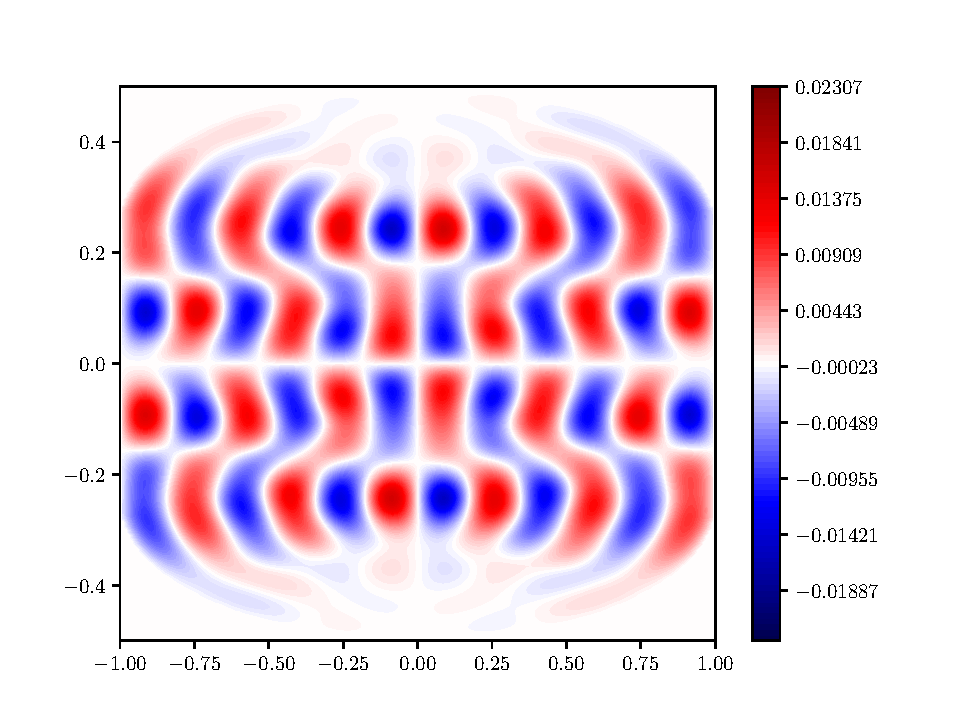
\includegraphics[width=\linewidth]{q6c-198.pdf}
          \caption*{$E_{198}= 755.8825724428713$}
        \end{minipage}
        \begin{minipage}{0.3\linewidth}
          \centering
          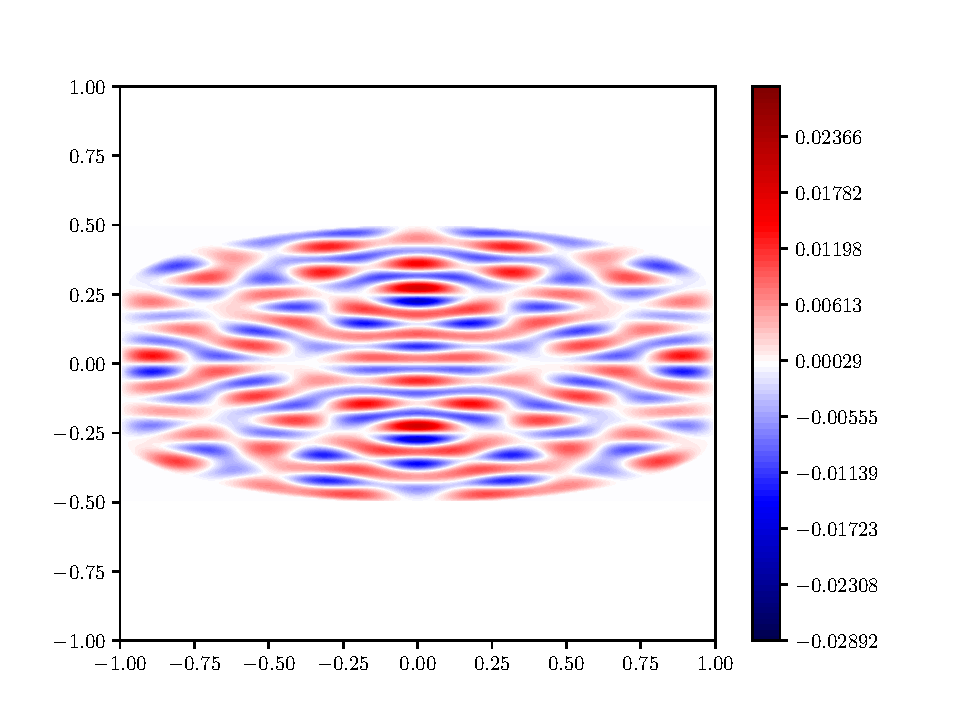
\includegraphics[width=\linewidth]{q6c-199.pdf}
          \caption*{$E_{199}= 757.6928364999236$}
        \end{minipage}
        \caption{Eigenstates and their eigenenergies for a 2-D potential well.}
        \label{fig:q6c-3}
      \end{figure}
    \end{enumerate}
  \end{enumerate}

\end{enumerate}

\end{document}


